

\section{Introduction}\label{sec:introduction_6}


Generative models have become increasingly popular in recent years due to their ability to capture complex data distributions and generate high-quality, realistic samples.
Not all model families permit efficient and accurate inference on both density estimation and sampling tasks. Indeed, the trade-offs in the inference capabilities of the current generative models have led to the development of very diverse approaches: Generative adversarial networks (GANs) \cite{goodfellow2020generative}, Variational Autoencoders (VAEs) \cite{kingma2013auto}, Energy-based models \cite{lecun2005loss} and Normalizing flows \cite{rezende2015variational}. 


% \section{Contributions}
\textbf{Normalizing flows} transform a simple probability distribution into a more complex one through a series of invertible transformations $f$.
The key defining property of flow-based generative models is that transformations $f$ must be \textbf{invertible} and both $f$ and $f^{-1}$ must be \textbf{differentiable}.
Normalizing flows based on coupling functions require a bijective one-dimensional function $h(z)$ and the derivative of the function with respect the input variable $z$ (also called the spatial dimension), i.e. $\frac{\partial h}{\partial z}$.
Related flows based on coupling layers such as NICE \cite{dinh2014nice} and RealNVP \cite{dinh2016density}, have an analytic one-pass inverse, but are often less flexible than their autoregressive counterparts. 

Based on these limitations, this work proposes to implement the \textbf{coupling function $h$ using the integration of continuous piecewise-affine (CPA) velocity functions} as a building block. A fully-differentiable module based on the integration of CPA velocity functions is presented, which yield diffeomorphic curves. Computing the inverse of such curves is equivalent to computing the forward curve backward in time or with opposite sign of the parameters. These diffeomorphic curves are used as the coupling function $h(z)$. 

The module acts as a \textbf{drop-in replacement for the affine or additive transformations} commonly found in coupling and autoregressive transforms. 
When combined with alternating invertible linear transformations, the resulting class of normalizing flows is referred to as \textbf{closed-form diffeomorphic spline flows} (DIFW-NF), which may feature coupling layers, DIFW-NF (C), or autoregressive layers, DIFW-NF (AR).
Overall, DIFW-NF resembles a traditional feed-forward neural network architecture, alternating between linear transformations and element-wise non-linearities, while retaining an exact, analytic inverse.
Experiments demonstrate that this module significantly enhances the flexibility of both classes of flows, obtaining competitive results in a variety of high-dimensional datasets.

The article is structured as follows: 
in \cref{sec:related_work} an extensive review of the coupling-based normalizing flows is presented. The proposed model is detailed in \cref{sec:method_6} and the experiments applied to 1D, 2D and ND data are included in \cref{sec:results_6}. Finally, conclusions are stated in \cref{sec:conclusions_6}.


\begin{figure}[!htb]
    \begin{center}
      \scalebox{1.0}{
      \begin{tikzpicture}
        \begin{scope}[shift={(0,0)}]
            \node[text width=4cm] at (0,0) {Generative direction \\ $\quad\quad \mathbf{z} \sim q(\mathbf{z})$ \\ $\quad\quad \mathbf{x} = f(\mathbf{z})$};
            \node[] at (6.5,0) {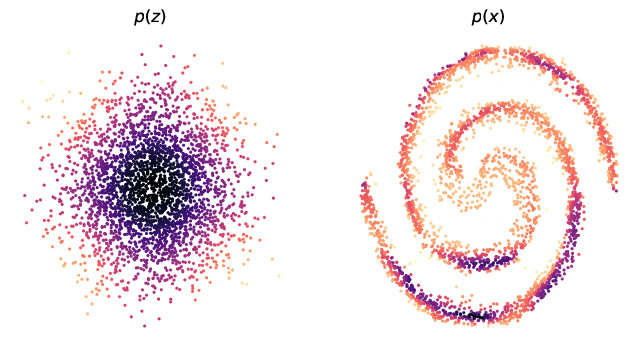
\includegraphics[width=0.6\linewidth,trim=0 0 0 25cm, clip]{figures/2D/plot_generative_flow.png}};
            \path[draw, -latex, very thick] (6,0) -- (7,0);
            \node[] at (4,-2.5) {Latent Space $q(\mathbf{z})$};
            \node[] at (9,-2.5) {Data Space $p(\mathbf{x})$};
        \end{scope}
        \begin{scope}[shift={(0,-6)}]
            \node[text width=4cm] at (0,0) {Normalizing direction \\ $\quad\quad \mathbf{x} \sim p(\mathbf{x})$ \\ $\quad\quad \mathbf{z} = f^{-1}(\mathbf{x})$};
            \node[] at (6.5,0) {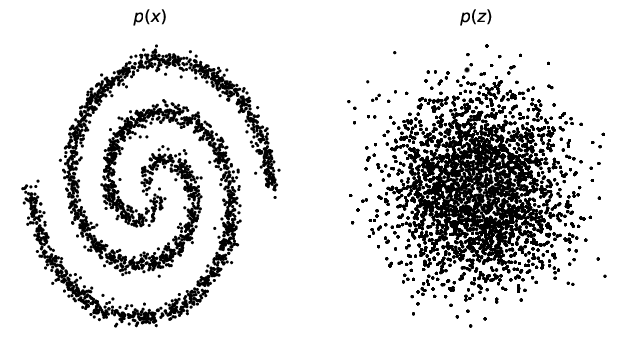
\includegraphics[width=0.6\linewidth,trim=0 0 0 25cm, clip]{figures/2D/plot_normalizing_flow.png}};
            \path[draw, -latex, very thick] (6,0) -- (7,0);
            \node[] at (4,-2.4) {Data Space $p(\mathbf{x})$};
            \node[] at (9,-2.4) {Latent Space $q(\mathbf{z})$};
        \end{scope}
        % \path[draw] (-2,-4) -- (13.5,-4);
      \end{tikzpicture}
      }
    \caption{Normalizing flow on a toy two-dimensional dataset. 
    The function $f(\mathbf{z})$ maps samples $\mathbf{z}$ from the latent distribution in the upper left into approximate samples $\mathbf{x}$ from the data distribution in the upper right. This corresponds to exact generation of samples from the model.
    The inverse function $f^{-1}(\mathbf{x})$ maps samples $\mathbf{x}$ from the data distribution in the lower left into approximate samples $\mathbf{z}$ from the latent distribution in the lower right. This corresponds to the exact inference of the latent state given the data. 
    }
    \label{fig:normalizing_flow_example_0}
    \end{center}
\end{figure}

\section{Related Work}\label{sec:related_work}

A normalizing flow is a transformation that converts a simple probability distribution $q(\mathbf{z})$  into a more complex one $p(\mathbf{x})$ by applying a sequence of invertible and differentiable mappings \cite{Papamakarios2021} (see \cref{fig:normalizing_flow_example_0}). 
There has been a growing interest in normalizing flows in the deep learning community, driven by successful applications and structural advantages they have over alternatives: \textbf{model flexibility} and \textbf{generation speed}. Normalizing flows can represent a richer family of distributions without requiring approximations. Flows have been explored both to increase the flexibility of the variational posterior in the context of VAEs, and directly as a generative model. 

\textbf{Autoregressive models} such as MAF \cite{papamakarios2017masked} achieve state-of-the-art density estimation performance on many challenging real-world datasets, but generally suffer from slow sampling time due to their autoregressive structure. These flows are $d$ times slower to invert than to evaluate, where $d$ is the dimensionality of $\mathbf{x}$. 
\textbf{Inverse autoregressive models} such as IAF \cite{kingma2016improved} can sample quickly and potentially have strong modeling capacity, but they cannot be trained efficiently by maximum likelihood.
Subsequent work which enhances the flexibility of autoregressive flows has resulted in models which do not have an analytic inverse, and require numerical optimization to invert. For instance, inverting the non-affine transformations used by NAF \cite{huang2018neural} and block-NAF \cite{de2020block} would require numerical optimization.
Transformations that are equally fast to invert and evaluate do exist. 
\textbf{Continuous flows} such as Neural ODEs \cite{chen2019neural} and FFJORD \cite{Grathwohl2019} are equally fast in both directions, but they require numerically integrating a differential equation in each direction, which can be slower than a single neural-network pass.

% Flows based on affine coupling layers such as NICE \cite{dinh2014nice} and RealNVP \cite{dinh2016density} only require a single neural-network pass in either direction, have an analytic one-pass inverse, but are often less flexible than their autoregressive counterparts, and as a result have so far lagged behind the latter models in density estimation benchmarks.


\textbf{Coupling flows} and autoregressive flows have a similar functional form and both have coupling functions as building blocks. A coupling function is a bijective differentiable function $\mathbf{h}(\cdot, \theta): \mathcal{R}^{d} \rightarrow \mathcal{R}^{d} $, parametrized by $\theta$. In coupling flows, these functions are typically constructed by applying a scalar coupling function $h(\cdot, \theta): \mathcal{R} \rightarrow \mathcal{R}$ element-wise. In autoregressive flows, $d = 1$ and hence they are also scalar valued. %Note that scalar coupling functions are necessarily (strictly) monotone. In this section we describe the scalar coupling functions commonly used in the literature.
\textbf{Additive and affine} coupling functions are used for coupling flows in NICE \cite{dinh2014nice}, RealNVP \cite{dinh2016density}, Glow \cite{kingma2018glow} and for autoregressive architectures in IAF and MAF. Both the affine and additive transformations are easy to invert, but they lack flexibility.
%Recalling that the base distribution of a flow is typically simple, flow-based models may struggle to model multi-modal or discontinuous densities using just affine or additive transformations, since they may find it difficult to compress and expand the density in a suitably nonlinear fashion. %This article aims to choose a more flexible function that is still differentiable and easy to invert.
\cite{ziegler2019latent} proposed an invertible \textbf{non-linear squared} transformation that adds an inverse-quadratic perturbation to an affine transformation in an autoregressive flow. 
The \textbf{Flow++ model} \cite{ho2019flow} uses the cumulative distribution function (CDF) of a mixture of logistic distributions as a monotonic transformation. In this case the computation of the inverse is done numerically with the bisection algorithm since a closed form is not available. The derivative of the transformation with respect to $z$ is expressed in terms of probability density function of logistic mixture.
Also related, \cite{Jaini2019} parametrize the monotonic transformation as a strictly increasing \textbf{sum of squares polynomial} (SOS).
For low-degree polynomials, an analytic inverse may be available, but the method would require an iterative solution in general. SOS is easier to train than NAF, because there are no restrictions on the parameters (like positivity of weights).

Regarding \textbf{linear splines}, 
\cite{muller2019neural} divided the domain into $k$ equal bins and modeled $h$ as the integral of a positive piecewise-constant function. 
\cite{muller2019neural} also used a \textbf{monotone quadratic spline} on the unit interval and modeled it as the integral of a positive piecewise-linear function. Such spline is invertible but finding its inverse requires solving a quadratic equation.
\cite{durkan2019cubic} proposed using \textbf{monotone cubic splines} defined only on the interval $[0,1]$. To ensure that the input is always between 0 and 1, a sigmoid transformation was placed before each coupling layer, and a logit transformation after each coupling layer.
% By composing coupling layers featuring element-wise monotonic cubic-spline transforms with invertible linear transformations, these flows are much more flexible than the standard coupling-layer models in the style of RealNVP, achieving similar results to autoregressive models on a suite of density-estimation tasks.
% Steffen's method \cite{steffen1990simple} is used to construct the spline. Here, one specifies $K + 1$ knots of the spline and boundary derivatives $\hat{h}'(0)$ and $\hat{h}'(1)$. These quantities are modelled as the output of a neural network. 
% Computation of the derivative is easy as it is piecewise-quadratic. 
A monotone cubic polynomial has only one real root and for inversion, one can find this either analytically or numerically. 
The flow can be trained by gradient descent by differentiating through the numerical root finding method. However, the procedure is numerically unstable if not treated carefully, as noted by \cite{durkan2019neural} when the sigmoid saturates for values far from zero, %: limitations of 32-bit floating point precision mean that in practice the sigmoid saturates for inputs outside the approximate range of [-13, 13]. 
Also related, 
\cite{durkan2019neural} model a coupling function as a \textbf{monotone rational-quadratic spline} on an interval and as the identity in the rest of the domain.
% They specify $K+1$ knots $(h_{x_{i}})_{i=0}^{K}$ and the derivatives at the inner points $(h'_{x_{i}})_{i=1}^{K-1}$, which are modelled as the output of a neural network. 
The derivative is a quotient derivative and the inverse is obtained by solving a quadratic equation. The RQ-NSF (C) coupling architecture and RQ-NSF(AR) autoregressive architectures used these coupling functions.


In the hope of creating an ideal likelihood-based generative model that simultaneously has fast sampling, fast inference, and strong density estimation performance, this article proposes replacing the conditional affine transformation \cite{kingma2016improved} with a more rich family of transformations, and note the requirements for doing so. In particular, we propose a novel normalizing-flow model based on a coupling function $h$ using the integration of continuous piecewise-affine velocity functions as a building block. Approaches like SOS \cite{Jaini2019}, cubic splines \cite{durkan2019cubic} and Flow++  \cite{ho2019flow} present couplings that are similar in spirit to our approach. 
% For instance, \cite{muller2019neural} found piecewise polynomial couplings to be more expressive than affine couplings, but reported little performance gains in density estimation. 
% The next section presents the details of the proposed method.

\section{Diffeomorphic Coupling Functions}\label{sec:method_6}

Normalizing flows based on coupling functions require a \textbf{bijective one-dimensional function} $h(z)$ and the derivative of the function with respect the input variable $z$ (also called the spatial dimension), i.e. $\frac{\partial h}{\partial z}$.
This work proposes a fully-differentiable module based on the \textbf{integration of continuous piecewise-affine (CPA) velocity functions}, which yield diffeomorphic curves $\phi^{\theta}(x,t)$ (differentiable, invertible and with differentiable inverse). As a matter of fact, computing the inverse is exactly the same as computing the forward curve backward in time or by flipping the sign of the parameters. These diffeomorphic curves will be used as the coupling function, so $h(z) = \phi^{\theta}(z,t)$. 
The diffeomorphic function itself maps an interval $[-B, B]$ to $[-B, B]$, as illustrated on \cref{fig:nf_simple3}. The transformation outside this range is defined as the identity, resulting in linear tails, so that the overall transformation can take unconstrained inputs.

\begin{figure}[!htb]
  \begin{center}
    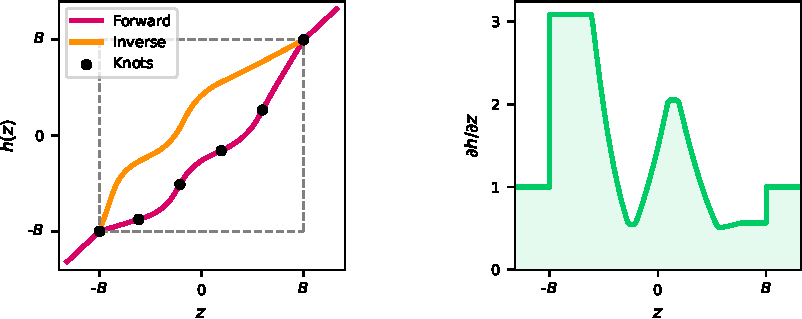
\includegraphics[width=\linewidth]{figures/nf_simple3.pdf}
    \caption{The proposed diffeomorphic transforms are drop-in replacements for additive or affine transformations in coupling or autoregressive layers, greatly enhancing their flexibility while retaining exact invertibility. 
    \textbf{Left}: Forward and inverse transformer of a random diffeomorphic monotonic function with tessellation size of 5 bins and linear tails, which is parametrized by a series of 6 points in the plane, and the 5 derivatives at the internal knots. \textbf{Right}: Transformer derivative with respect to $z$. }
    \label{fig:nf_simple3}
  \end{center}
  \vspace{-0.5cm}
\end{figure}

The module acts as a \textbf{drop-in replacement for the affine or additive transformations} commonly found in coupling and autoregressive transforms. 
Unlike the additive and affine transformations, which have limited flexibility, the proposed differentiable monotonic function with sufficiently many intervals can approximate any differentiable monotonic function on the specified interval $[-B, B]$, yet has a closed-form, tractable Jacobian determinant, and can be inverted analytically. The proposed parameterization is fully-differentiable, which allows for training by gradient methods.

The proposed formulation can also easily be adapted for autoregressive transforms; each $\theta_{k}$ can be computed as a function of $\mathbf{z}_{1:i}$ using an autoregressive neural network, and then all elements of $\mathbf{z}$ can be transformed at once. %Inspired by this, we also introduce a set of splines for our coupling layers which act element-wise on $\mathbf{z}_{1:i}$, and whose parameters are optimized directly by stochastic gradient descent.
When combined with alternating invertible linear transformations, the resulting class of normalizing flows is referred to as \textbf{closed-form diffeomorphic spline flows (DIFW-NF)}, which may feature coupling layers, DIFW-NF (C), or autoregressive layers, DIFW-NF (AR).
Experiments demonstrate that this module significantly \textbf{enhances the flexibility} of both classes of flows, and in some cases brings the performance of coupling transforms on par with the best-known autoregressive flows.
DIFW-NF only requires a single neural-network pass in either the forward or the inverse direction, but in practice is as flexible as state-of-the-art autoregressive flows.
% These diffeomorphic functions are easily differentiable and also analytically invertible. Nevertheless, they are strictly more flexible than quadratic functions, and allow direct parameterization of the derivatives and heights at each knot.
Overall, DIFW-NF resembles a traditional feed-forward neural network architecture, alternating between linear transformations and element-wise non-linearities, while retaining an exact, analytic inverse.
Like Real NVP or Glow, DIFW-NF flows can represent either a transformation from data to noise, or from noise to data. In both cases, the transformation requires only a single pass of the neural network defining the flow.
Note that for the rest of the section the spatial dimension of the transformation will be referred to as $x$ instead of $z$.


\subsection{CPA-based Diffeomorphic Transformations}

Let's recall the CPA-based diffeomorphic transformations introduced in \cite{martinez2022closed}. A diffeomorphism can be obtained, via integration, from uniformly continuous stationary velocity fields $T^{\theta}(x) = \phi^{\theta}(x,1)$ 
where $\phi^{\theta}(x,t) = x + \int_0^t v^{\theta}(\phi^{\theta}(x,\tau)) d\tau$ for uniformly continuous $v: \Omega \rightarrow \mathbb{R}$ and integration time $t$. 
Here $x$ refers to the spatial dimension and $t$ the integration time.
The solution for the integral equation is a composition of a finite number of solutions $\psi$, given by: $\phi^\theta(x,t) = \big(\psi_{\theta,c_m}^{t_m} \circ \psi_{\theta,c_{m-1}}^{t_{m-1}} \circ \cdots \circ \psi_{\theta,c_2}^{t_2} \circ \psi_{\theta,c_1}^{t_1} \big)(x)$, 
where $m$ is the number of cells visited and $\psi_{\theta,c}^{t}$ is the solution of a basic ODE $\frac{d\psi}{dt}=v^\theta(\psi)$
with an $\mathbb{R} \rightarrow \mathbb{R}$ affine velocity field: 
$v^\theta(\psi) = a^\theta \psi + b^\theta$ and an initial condition $\psi(x,0) = x$.

During the iterative process of integration, several cells are crossed, starting from $c_1$ at integration time $t_1=1$, and finishing at $c_m$ at integration time $t_m$. The integration time $t_m$ of the last cell $c_m$ can be calculated by subtracting from the initial integration time the accumulated boundary hitting times $t_{hit}$: $t_m = t_1 - \sum_{i=1}^{m-1} t_{hit}^\theta(c_i, x_i)$. The final integration point $x_m$ is the boundary of the penultimate cell $c_{m-1}$: $x_m = x_{c_{m-1}}$. In case only one cell is visited, both time and space remain unchanged: $t_m = 1$ and $x_m = x$. Taking this into consideration, the trajectory can be calculated as follows:
\begin{equation}\label{eq:closed_form_integration:repeat}
\phi^\theta(x,t) = \psi^\theta(x=x_m,t=t_m) = 
\bigg(
    x e^{t a_c} + \Big(e^{t a_c}-1\Big) \frac{b_c}{a_c}
\bigg)_{\substack{x = x_m \\ t = t_m}}
\end{equation}
Gradient-based optimization algorithms require the derivatives of the transformation with respect to the model parameters $\theta$ and $x$. That is, we need to obtain: 
\begin{itemize}
  \item $\color{Magenta}\boxed{\color{black}\cfrac{\partial \phi^\theta(x,t)}{\partial \theta}}$: partial derivative of transformation $\phi^\theta(x,t)$ w.r.t. $\theta$. Presented at \cite{martinez2022closed}.
  \item $\color{Violet}\boxed{\color{black}\cfrac{\partial \phi^\theta(x,t)}{\partial x}}$: partial derivative of transformation $\phi^\theta(x,t)$ w.r.t. $x$.
\end{itemize}


The closed-form derivative ${\partial \phi^\theta(x,t)}/{\partial \theta}$ was presented in \cite{martinez2022closed}. 
% Here the derivative ${\partial \phi^\theta(x,t)}/{\partial x}$ w.r.t. the spatial variable is also required.
In addition, a normalizing flow model involves computing the Jacobian determinant, so under gradient-based optimization techniques, second order derivatives are also required:
\begin{itemize}
  \item  $\color{ForestGreen}\boxed{\color{black}\cfrac{\partial^2 \phi^\theta(x,t)}{\partial x^2}}$: partial second derivative of transformation $\phi^\theta(x,t)$ w.r.t. $x$.
  \item  $\color{Orange}\boxed{\color{black}\cfrac{\partial^2 \phi^\theta(x,t)}{\partial x \partial \theta}}$: partial second derivative of transformation $\phi^\theta(x,t)$ w.r.t. $x$ and $\theta$.
\end{itemize}


\subsection{Closed-Form Derivatives of $\phi^\theta(x,t)$ w.r.t. $x$}\label{sec:closed_form_derivative_x}

The derivative can be calculated by going backwards in the integration direction. We focus on the partial derivative w.r.t. the spatial dimension $x$, and derive each of the terms of this derivative:
\begin{equation}
\color{Violet}\boxed{\color{black}\frac{\partial \phi^\theta(x,t)}{\partial x}}\color{black} = 
\bigg(
\frac{\partial \psi^\theta(x,t)}{\partial x} + 
\frac{\partial \psi^\theta(x,t)}{\partial t^\theta} \cdot
\frac{\partial t^\theta}{\partial x}
\bigg)_{\substack{x = x_m \\ t = t_m}}
\end{equation}

% Let's derive each of the terms of this derivative:
% \begin{center}
% $\cfrac{\partial \psi^\theta(x,t)}{\partial x}\;,\;$
% $\cfrac{\partial \psi^\theta(x,t)}{\partial t^\theta}\;,\;$ 
% $\cfrac{\partial t^\theta}{\partial x}$.
% \end{center}

\subsubsection{Expression for $\cfrac{\partial \psi^\theta(x,t)}{\partial x}$}

Based on the expression for $\psi(x,t)$ from \cref{eq:closed_form_integration:repeat}, 
% \begin{equation}
% \psi^\theta(x,t) = x e^{t a_c} + \Big(e^{t a_c}-1\Big) \frac{b_c}{a_c}
% \end{equation}
we can obtain the derivative w.r.t. $x$:
\begin{equation}
\phi^\theta(x,t) = \psi^\theta(x=x_m,t=t_m) = 
  \bigg(
      x e^{t a_c} + \Big(e^{t a_c}-1\Big) \frac{b_c}{a_c}
  \bigg)_{\substack{x = x_m \\ t = t_m}}
\end{equation}
It is important to note that the variable $x$ only affects this expression when $m=1$, otherwise is zero. That is, when the integration process does not traverse to adjacent cells 
% (see \cref{fig:integration_process_grid}) 
the value of $x$ is present on $\phi^\theta(x,t)$, otherwise is $x_m$. Here $\indicator{C}$ is the indicator function that takes value 1 when the condition $C$ is true.
\begin{equation}
  \frac{\partial \psi^\theta(x,t)}{\partial x} = %\big(e^{t a_c}\big)_{x_{m}=x}
  e^{t a_c} \cdot \indicator{m=1} %\bigg|_{m=1}
\end{equation}


\subsubsection{Expression for $\cfrac{\partial \psi^\theta(x,t)}{\partial t^\theta}$}

Similarly, from the same expression for $\psi(x,t)$,
% \begin{equation}
% \psi^\theta(x,t) = x e^{t a_c} + \Big(e^{t a_c}-1\Big) \frac{b_c}{a_c}
% \end{equation}
we explicitly get the derivative w.r.t $t^\theta$:
\begin{equation}\label{eq:psi_derivative_t:repeated}
    \frac{\partial \psi^\theta(x,t)}{\partial t^\theta} = x \, a_c \, e^{t a_c} + a_c \, e^{t a_c} \frac{b_c}{a_c} = 
    e^{t a_c} \big( a_c x + b_c \big)
\end{equation}


\subsubsection{Expression for $\cfrac{\partial t^\theta}{\partial x}$}


After visiting $m$ cells, the integration time $t^\theta$ can be expressed as:
\begin{equation}\label{eq:time:repeated}
t^\theta = t_1 - \sum_{i=1}^{m-1} t_{hit}^\theta(c_i, x_i)
\end{equation}
In this case, the variable $x$ only affects \cref{eq:time:repeated} if we move away from the first cell, i.e. $m>1$, and on the first cell $c=1$, which results the following expresion:
\begin{equation}\label{eq:time_derivative_x}
\frac{\partial t^\theta}{\partial x} = 
-\sum_{i=1}^{m-1} \frac{\partial t_{hit}^\theta(c_i, x_i)}{\partial x} = 
  -\cfrac{\partial t_{hit}^\theta(c, x)}{\partial x} \cdot \indicator{m>1} %\bigg|_{m>1}
\end{equation}
where
\begin{equation}\label{eq:thit:repeat}
t_{hit}^\theta(c, x) = \frac{1}{a_c} \log \bigg( \frac{a_c x_c + b_c}{a_c x + b_c} \bigg)
\end{equation}
and $x_c$ is the boundary for cell index $c$. Now, apply the chain rule operation to the hitting time $t_{hit}^\theta(c, x)$ expression:
\begin{equation}\label{eq:thit_derivative_x}
\frac{\partial t_{hit}^\theta(c, x)}{\partial x} = 
\frac{1}{a_c} \frac{-a_{c}\cfrac{a_c x_c + b_c}{(a_c x + b_c)^2}}{\cfrac{a_c x_c + b_c}{a_c x + b_c}} = 
\frac{-1}{a_c x + b_c}
\end{equation}
Then, based on \cref{eq:time_derivative_x}, the derivative of the integration time $t^\theta$ can be expressed as:
\begin{equation}\label{eq:time_derivative_x_final}
\frac{\partial t^\theta}{\partial x} = %\sum_{i=1}^{m-1} \frac{1}{a_{c_i} x_i + b_{c_i}}
-\cfrac{\partial t_{hit}^\theta(c, x)}{\partial x} \cdot \indicator{m>1} = %\bigg|_{m>1} = 
\cfrac{1}{a_c x + b_c} \cdot \indicator{m>1} %\bigg|_{m>1}
\end{equation}

\subsubsection{Final Expression for $\color{Violet}\boxed{\color{black}\cfrac{\partial \phi^\theta(x,t)}{\partial x}}$}

Joining all the terms together and evaluating the derivative at $x = x_m$ and $t = t_m$ yields the expression for the partial derivative w.r.t. $x$:

\begin{equation}\label{eq:derivative_x_complete}
\begin{aligned}
  \frac{\partial \phi^\theta(x,t)}{\partial x} &= 
  \bigg(
  \frac{\partial \psi^\theta(x,t)}{\partial x} + 
  \frac{\partial \psi^\theta(x,t)}{\partial t^\theta} \cdot
  \frac{\partial t^\theta}{\partial x}
  \bigg)_{\substack{x = x_m \\ t = t_m}} = \\ &= 
  % e^{t_m a_{c_m}}  \bigg|_{m=1}  + e^{t_m a_{c_m}} \cfrac{a_{c_m} x_m + b_{c_m}}{a_c x + b_c}  \bigg|_{m>1} = \\ &=
  e^{t_m a_{c_m}} \cdot \indicator{m=1}  + e^{t_m a_{c_m}} \cfrac{a_{c_m} x_m + b_{c_m}}{a_c x + b_c}  \cdot \indicator{m>1} = \\ &=
  \left\{\begin{array}{ll}
    e^{t_m a_{c_m}} \cfrac{a_{c_m} x_m + b_{c_m}}{a_c x + b_c} & \text{if} \quad m>1\\ 
    e^{t_m a_{c_m}} & \text{otherwise}
    \end{array}\right.
\end{aligned}
\end{equation}


\subsection{Closed-Form Derivatives of $\cfrac{\partial \phi^\theta(x,t)}{\partial x}$ w.r.t. $x$}\label{sec:closed_form_derivative_x_x}


In this case, we start from the previous \cref{eq:derivative_x_complete} and derive again w.r.t. $x$:

\begin{equation}
  \color{ForestGreen}\boxed{\color{black}\frac{\partial^2 \phi^\theta(x,t)}{\partial x^2}}\color{black} = 
  \bigg(
  \frac{\partial^2 \psi^\theta(x,t)}{\partial x^2} + 
  \frac{\partial^2 \psi^\theta(x,t)}{\partial x \, \partial t^\theta} \cdot
  \frac{\partial t^\theta}{\partial x} + 
  \frac{\partial \psi^\theta(x,t)}{\partial t^\theta} \cdot
  \frac{\partial^2 t^\theta}{\partial x^2}
  \bigg)_{\substack{x = x_m \\ t = t_m}}
\end{equation}

\subsubsection{Expression for $\cfrac{\partial^2 \psi^\theta(x,t)}{\partial x^2}$}

\begin{equation}
\frac{\partial^2 \psi^\theta(x,t)}{\partial x^2} = 
\frac{\partial}{\partial x}\Big(\frac{\partial \psi^\theta(x,t)}{\partial x}\Big) = 
% \frac{\partial}{\partial x}\Big(e^{t a_c}\big|_{m>1}\Big) = 0
\frac{\partial}{\partial x}\Big(e^{t a_c}\cdot \indicator{m>1}\Big) = 0
\end{equation}

\subsubsection{Expression for $\cfrac{\partial^2 \psi^\theta(x,t)}{\partial t^\theta \partial x}$}

\begin{equation}
  \frac{\partial^2 \psi^\theta(x,t)}{\partial t^\theta \partial x} = 
  \frac{\partial}{\partial x}\Big(\frac{\partial \psi^\theta(x,t)}{\partial t^\theta}\Big) = 
  \frac{\partial}{\partial x}\Big(e^{t a_c} \big( a_c x + b_c \big)\Big) = e^{t a_c} a_c
\end{equation}

\subsubsection{Expression for $\cfrac{\partial^2 t^\theta}{\partial x^2}$}

Again, in this case the variable $x$ only affects \cref{eq:time:repeated} if we move away from the first cell, i.e. $m>1$, and on the first cell $c=1$:

\begin{equation}
  \frac{\partial^2 t^\theta}{\partial x^2} = 
  \frac{\partial}{\partial x}\Big(\frac{\partial  t^\theta}{\partial x}\Big) = 
  \frac{\partial}{\partial x} \cfrac{1}{a_c x + b_c} \cdot \indicator{m>1} = %\bigg|_{m>1} =
  - \frac{a_{c}}{(a_{c} x + b_{c})^2} \cdot \indicator{m>1} %\bigg|_{m>1}
\end{equation}

\subsubsection{Final Expression for $\color{ForestGreen}\boxed{\color{black}\cfrac{\partial^2 \phi^\theta(x,t)}{\partial x^2}}$}

Joining all the terms together and evaluating the derivative at $x = x_m$ and $t = t_m$ yields the expression for the partial derivative w.r.t. $x$:

\begin{equation}\label{eq:derivative_x2_complete}
\begin{aligned}
  \frac{\partial^2 \phi^\theta(x,t)}{\partial x^2} &= 
  \bigg(
  \frac{\partial^2 \psi^\theta(x,t)}{\partial x^2} + 
  \frac{\partial^2 \psi^\theta(x,t)}{\partial t^\theta \partial x} \cdot
  \frac{\partial t^\theta}{\partial x} + 
  \frac{\partial \psi^\theta(x,t)}{\partial t^\theta} \cdot
  \frac{\partial^2 t^\theta}{\partial x^2}
  \bigg)_{\substack{x = x_m \\ t = t_m}} = \\ &=
  e^{t_m a_{c_m}} a_{c_m} \cfrac{1}{a_c x + b_c} \cdot \indicator{m>1} - %\bigg|_{m>1} - 
  e^{t_m a_{c_m}} \big( a_{c_m} x_m + b_{c_m} \big) \frac{a_{c}}{(a_{c} x + b_{c})^2} \cdot \indicator{m>1} %\bigg|_{m>1}
  % e^{t a_c} a_c \cdot \sum_{i=1}^{m-1} \frac{1}{a_{c_i} x_i + b_{c_i}} - 
  % e^{t a_c} \big( a_c x + b_c \big) \cdot \sum_{i=1}^{m-1} \frac{a_{c_i}}{(a_{c_i} x_i + b_{c_i})^2} 
\end{aligned}
\end{equation}





\subsection{Closed-Form Derivatives of $\cfrac{\partial \phi^\theta(x,t)}{\partial x}$ w.r.t. $\theta$}\label{sec:closed_form_derivative_x_theta}

We start from \cref{eq:derivative_x_complete} and derive w.r.t. one of the coefficients of $\theta$, i.e., $\theta_k$:
\begin{equation}
  \color{Orange}\boxed{\color{black}\frac{\partial^2 \phi^\theta(x,t)}{\partial \theta_k \, \partial x}}\color{black} = 
  \bigg(
  \frac{\partial^2 \psi^\theta(x,t)}{\partial \theta_k \, \partial x} + 
  \frac{\partial^2 \psi^\theta(x,t)}{\partial \theta_k \partial t^\theta} \cdot
  \frac{\partial t^\theta}{\partial x} + 
  \frac{\partial \psi^\theta(x,t)}{\partial t^\theta} \cdot
  \frac{\partial^2 t^\theta}{\partial \theta_k \partial x}
  \bigg)_{\substack{x = x_m \\ t = t_m}}
\end{equation}
Note that the slope $a_c$ and intercept $b_c$ are a linear combination of the orthogonal basis $B$ of the constraint matrix $L$, with $\theta$ as coefficients. 
% We recommend the reader to review \cref{sec:velocity_continuity_constraints,sec:null_space} for more information about these matrices.
\begin{equation}\label{eq:vec_A:repeat}
vec(\textbf{A}) = \textbf{B} \cdot \boldsymbol{\theta} = \sum_{j=1}^{d} \theta_j \cdot \textbf{B}_j
\end{equation}
If we define one of the components from the orthogonal basis $\textbf{B}_j$ as:
\begin{equation}\label{eq:basis:repeat}
\textbf{B}_{j} = \begin{bmatrix} a_1^{(j)} & b_1^{(j)} & \cdots & a_c^{(j)} & b_c^{(j)} & \cdots & a_{N_\mathcal{P}}^{(j)} & b_{N_\mathcal{P}}^{(j)}\end{bmatrix}^T
\end{equation}
Then,
\begin{equation}\label{eq:vec_A_complete:repeat}
vec(\textbf{A}) = \sum_{j=1}^{d} \theta_j \cdot \textbf{B}_j = \begin{bmatrix} & \cdots & \sum_{j=1}^{d} \theta_j a_c^{(j)} & \sum_{j=1}^{d} \theta_j b_c^{(j)} & \cdots & \end{bmatrix}^T
\end{equation}
Thus, the slope $a_c$ and intercept $b_c$ (parameters of the affine transformation) and their derivatives w.r.t. one of the coefficients of $\theta$, i.e., $\theta_k$, are denoted as follows:
\begin{equation}\label{eq:ac_bc:repeat}
a_c = \sum_{j=1}^{d} \theta_j a_c^{(j)} \quad\quad\quad
b_c = \sum_{j=1}^{d} \theta_j b_c^{(j)}
\end{equation}
\begin{equation}\label{eq:ac_bc_partial}
  \frac{\partial a_c}{\partial \theta_k} = a_c^{(k)} \quad\quad\quad
  \frac{\partial b_c}{\partial \theta_k} = b_c^{(k)}
  \end{equation}

\subsubsection{Expression for $\cfrac{\partial^2 \psi^\theta(x,t)}{\partial \theta_k \, \partial x}$}

Given that $\cfrac{\partial \psi^\theta(x,t)}{\partial x} = e^{t a_c} \cdot \indicator{m=1}$, we derive w.r.t. one of the coefficients of $\theta$, i.e., $\theta_k$:

\begin{equation}
\frac{\partial^2 \psi^\theta(x,t)}{\partial \theta_k \, \partial x} =
\frac{\partial^2 \psi^\theta(x,t)}{\partial a_c \, \partial x} \cdot \frac{\partial a_c}{\partial \theta_k} = 
t \cdot e^{t a_c} \cdot \indicator{m=1} \cdot a_c^{(k)} 
\end{equation}

\subsubsection{Expression for $\cfrac{\partial^2 \psi^\theta(x,t)}{\partial \theta_k \partial t^\theta}$}

Given that $\cfrac{\partial \psi^\theta(x,t)}{\partial t^\theta} = e^{t a_c} \big( a_c x + b_c \big)$, we derive w.r.t. one of the coefficients of $\theta$, i.e., $\theta_k$:
\begin{equation}\label{eq:derivative_phi_x_thetak}
  \frac{\partial^2 \psi^\theta(x,t)}{\partial \theta_k \, \partial t^\theta} =
  \frac{\partial^2 \psi^\theta(x,t)}{\partial {t^\theta} \, \partial t^\theta} \cdot \frac{\partial t^\theta}{\partial \theta_k} +
  \frac{\partial^2 \psi^\theta(x,t)}{\partial a_c \, \partial t^\theta} \cdot \frac{\partial a_c}{\partial \theta_k} +
  \frac{\partial^2 \psi^\theta(x,t)}{\partial b_c \, \partial t^\theta} \cdot \frac{\partial b_c}{\partial \theta_k}
\end{equation}
We reutilize $\cfrac{\partial t^\theta}{\partial \theta_k}$ from \cite{martinez2022closed}, and derive each remaining term.
\begin{equation}\label{eq:derivative_t_t}
\frac{\partial^2 \psi^\theta(x,t)}{\partial {t^\theta} \, \partial t^\theta} = 
e^{t a_c} ( a_c x + b_c) \cdot a_c
\end{equation}
\begin{equation}\label{eq:derivative_t_a}
\frac{\partial^2 \psi^\theta(x,t)}{\partial a_c \, \partial t^\theta} = 
\frac{\partial}{\partial a_c}\bigg( e^{t a_c} ( a_c x + b_c) \bigg) = 
t e^{t a_c} (a_c x + b_c) + e^{t a_c} x = 
e^{t a_c} (t(a_c x + b_c) + x)
\end{equation}
\begin{equation}\label{eq:derivative_t_b}
\frac{\partial^2 \psi^\theta(x,t)}{\partial b_c \, \partial t^\theta} = 
\frac{\partial}{\partial b_c}\bigg( e^{t a_c} ( a_c x + b_c) \bigg) = 
e^{t a_c} 
\end{equation}

% Therefore, joining the expressions from \cref{eq:thit_derivative_theta_final,eq:derivative_t_t,eq:derivative_t_a,eq:derivative_t_b} into \cref{eq:derivative_phi_x_thetak}:
Therefore, joining the expressions from \cref{eq:derivative_t_t,eq:derivative_t_a,eq:derivative_t_b} into \cref{eq:derivative_phi_x_thetak}:
\begin{equation}
\begin{aligned}
\frac{\partial^2 \psi^\theta(x,t)}{\partial \theta_k \, \partial t^\theta} =
e^{t a_c} ( a_c x + b_c) a_c \cdot \frac{\partial t^\theta}{\partial \theta_k} + 
e^{t a_c} (t(a_c x + b_c) + x) \cdot a_c^{(k)} + 
e^{t a_c}  \cdot b_c^{(k)}
\end{aligned}
\end{equation}


\subsubsection{Expression for $\cfrac{\partial^2 t^\theta}{\partial \theta_k \partial x}$}


Given that $\cfrac{\partial t^\theta}{\partial x} = \cfrac{1}{a_c x + b_c}  \cdot \indicator{m>1}$, we derive w.r.t. one of the coefficients of $\theta$, i.e., $\theta_k$:

\begin{equation}
  \begin{aligned}  
    \frac{\partial^2 t^\theta}{\partial \theta_k \, \partial x} &=
    \frac{\partial^2 t^\theta}{\partial a_c \, \partial x} \cdot \frac{\partial a_c}{\partial \theta_k} +
    \frac{\partial^2 t^\theta}{\partial b_c \, \partial x} \cdot \frac{\partial b_c}{\partial \theta_k} = \\ &=
    \frac{-x}{(a_c x + b_c)^2}\cdot a_c^{(k)} + 
    \frac{-1}{(a_c x + b_c)^2}\cdot b_c^{(k)}
\end{aligned}
\end{equation}

\subsubsection{Final Expression for $\color{Orange}\boxed{\color{black}\cfrac{\partial^2 \phi^\theta(x,t)}{\partial \theta_k \, \partial x}}$}

Joining all the terms together and evaluating the derivative at $x = x_m$ and $t = t_m$ yields the expression for the partial derivative w.r.t. $x$
% \footnote{Dear reader, if you have made it this far, you deserve some praise.
\includegraphics[height=1em]{figures/1F44F_color.png}}
:
\begin{equation}
\begin{aligned}
  \frac{\partial^2 \phi^\theta(x,t)}{\partial \theta_k \, \partial x} &= 
  \bigg(
  \frac{\partial^2 \psi^\theta(x,t)}{\partial \theta_k \, \partial x} + 
  \frac{\partial^2 \psi^\theta(x,t)}{\partial \theta_k \partial t^\theta} \cdot
  \frac{\partial t^\theta}{\partial x} + 
  \frac{\partial \psi^\theta(x,t)}{\partial t^\theta} \cdot
  \frac{\partial^2 t^\theta}{\partial \theta_k \partial x}
  \bigg)_{\substack{x = x_m \\ t = t_m}} = \\ &= 
  t \cdot e^{t a_c} \cdot \indicator{m=1} \cdot a_c^{(k)} + \\
  &\quad\, \Big (
  e^{t a_c} ( a_c x + b_c) a_c \cdot \frac{\partial t^\theta}{\partial \theta_k} + 
  e^{t a_c} (t(a_c x + b_c) + x) \cdot a_c^{(k)} + 
  e^{t a_c}  \cdot b_c^{(k)} 
  \Big) \cdot
  \cfrac{1}{a_c x + b_c}  \cdot \indicator{m>1} + \\
  &\quad\, e^{t a_c} ( a_c x + b_c ) \cdot
  \Big (
  \frac{-x}{(a_c x + b_c)^2}\cdot a_c^{(k)} + 
  \frac{-1}{(a_c x + b_c)^2}\cdot b_c^{(k)}
  \Big )
\end{aligned}
\end{equation}




\section{Experiments and Results}\label{sec:results_6}

The performance of DIFW-NF flows were evaluated on both synthetic and real-world datasets for density estimation, and compare it to several alternative autoregressive models and flow based methods.
For these experiments, we define the forward and backward operators of the proposed normalizing flow model. The forward (generative) direction samples data $\mathbf{z}$ from a known distribution  $p(\mathbf{z})$ and applies a transformation $f$ to generate data samples $\mathbf{x} = f(\mathbf{z})$.
Similarly, the backward (normalizing) direction takes real data samples  $\mathbf{x} \sim p(\mathbf{x})$ and applies the inverse transformation $f^{-1}$. Model's loss function is simply the negative log-likelihood. 
% it is competitive with autoregressive models

\subsection{1-dimensional Data}
% \subsection{Simulated Experiments}

First, we performed a host of experiments on one-dimensional simulated data to gain in-depth understanding of DIFW-NF. Five datasets are tested: 
\textsc{blobs} generates isotropic one-dimensional Gaussian blobs,
\textsc{gaussian} creates an unimodal Gaussian distribution,
\textsc{gaussianmix} generates multimodal data from a mixture of Gaussians,
\textsc{power} applies the power transformation $5^x$
and \textsc{uniform} samples from a uniform 0-1 distribution. 




A grid-hyperparameter search is conducted for each dataset. 
Flows can be composed after $1$,$2$ or $3$ steps and the transformation tessellation size is chosen among $\{4,8,16,32\}$.
The Adam optimizer \cite{kingma2014adam} is used with default hyperparameters and an initial learning rate of $\{1e^{-4}, 1e^{-3}, 5e^{-3}\}$ over $500$ training epochs with batch size $256$. For training and test, $5000$ and $2000$ data points are used respectively. 
The final hyperparameters are shown in \cref{tab:nf_1d}, along with the log-likelihood of the generated data.


\begin{table}[!htb]
  \small
  \caption{Hyperparameters and log-probability for density-estimation results in 1D-datasets}
  \label{tab:nf_1d}
  \begin{center}
  \begin{tabular}{llllll}
    \toprule
    Dataset & \textsc{blobs} & \textsc{gaussian} & \textsc{gaussianmix} & \textsc{power} & \textsc{uniform} \\
    \midrule
    Train Size           &              5000 &              5000 &              5000 &             5000 &             5000 \\
    Test Size            &              2000 &              2000 &              2000 &             2000 &             2000 \\
    Batch Size           &               256 &               256 &               256 &              256 &              256 \\
    Tessellation Size    &                32 &                32 &                32 &                8 &               32 \\
    Flow Steps           &                 2 &                 2 &                 2 &                3 &                2 \\
    Epochs               &               500 &               500 &               500 &              500 &              500 \\
    Learning Rate        &             0.005 &             0.005 &             0.001 &            0.005 &            0.005 \\ \midrule
    $\log p(\mathbf{x})$ &  -3.70 $\pm$ 0.22 &  -1.49 $\pm$ 0.08 &  -1.22 $\pm$ 0.14 &  0.80 $\pm$ 0.02 &  0.01 $\pm$ 0.01 \\
    \bottomrule
    \end{tabular}    
  \end{center}
\end{table}

\begin{figure}[!htb]
    \begin{center}
    % \begin{subfigure}[b]{0.32\linewidth}
    % 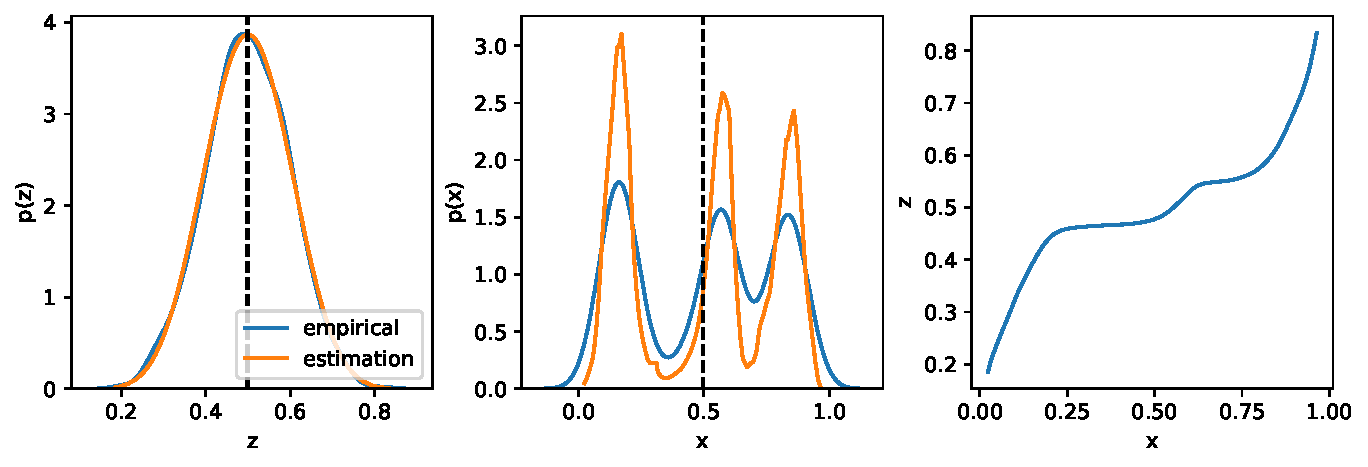
\includegraphics[width=\linewidth, trim=32 35 445 0, clip]{figures/1D/BLOBS/plot_1D.pdf}
    % \caption{Base distribution $q(\mathbf{z})$}
    % \end{subfigure}
    % \hfill
    % \begin{subfigure}[b]{0.32\linewidth}
    % 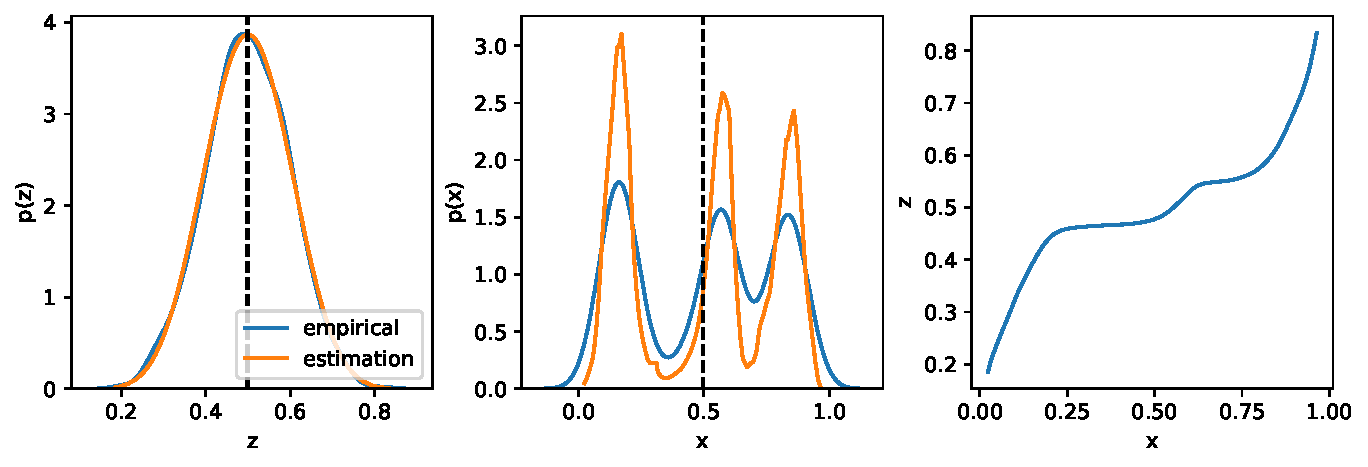
\includegraphics[width=\linewidth, trim=463 35 15 0, clip]{figures/1D/BLOBS/plot_1D.pdf}
    % \caption{Transformation $f(\mathbf{z})$}
    % \end{subfigure} 
    % \hfill
    % \begin{subfigure}[b]{0.32\linewidth}
    % 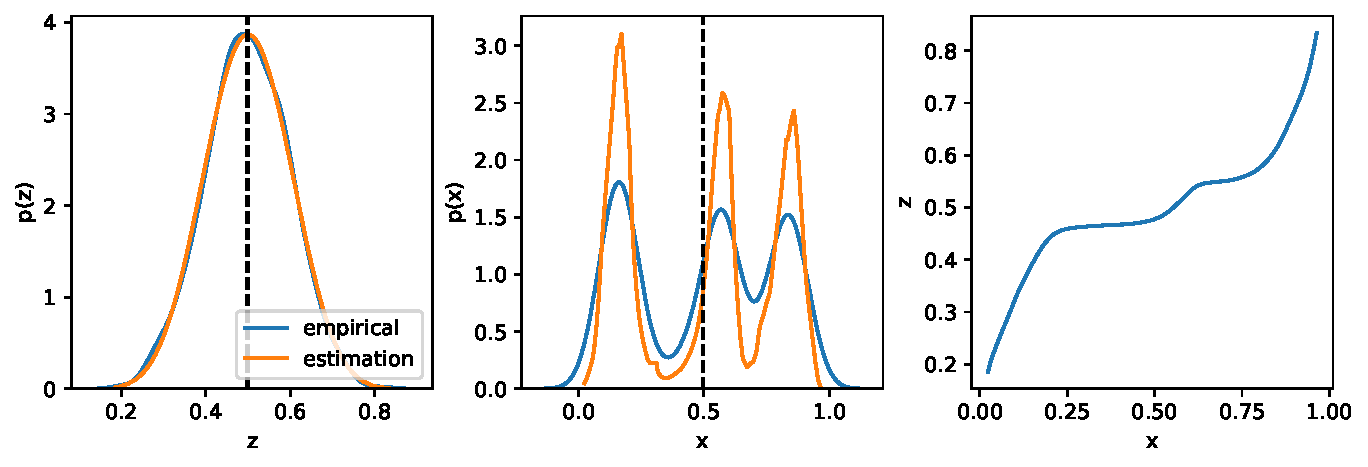
\includegraphics[width=\linewidth, trim=245 35 232 0, clip]{figures/1D/BLOBS/plot_1D.pdf}
    % \caption{Target distribution $p(\mathbf{x})$}
    % \end{subfigure} 
    % \\
    \begin{subfigure}[b]{0.48\linewidth}
    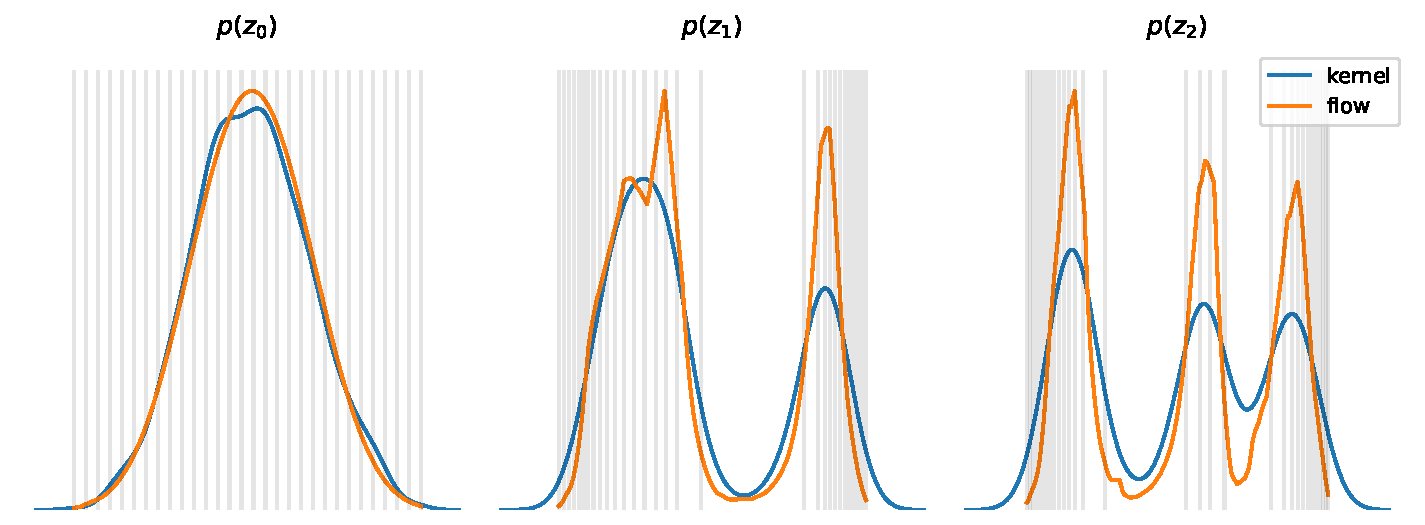
\includegraphics[width=\linewidth, trim=0 0 0 20, clip]{figures/1D/BLOBS/plot_generative_flow_evolution.pdf}
    \caption{Generative flow: noise $\Rightarrow$ data}
    \label{fig:nf_1d_example:generative}
    \end{subfigure}
    \hfill{\color{lightgray}\vrule}\hfill
    \begin{subfigure}[b]{0.48\linewidth}
    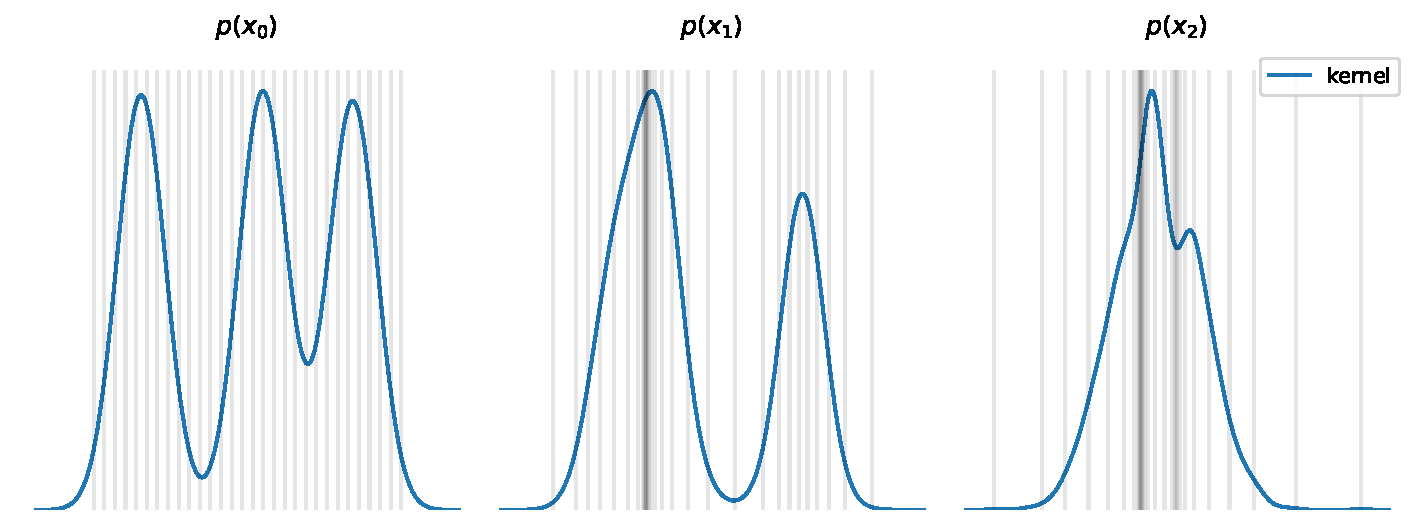
\includegraphics[width=\linewidth, trim=0 0 0 26, clip]{figures/1D/BLOBS/plot_normalizing_flow_evolution.pdf}
    \caption{Normalizing flow: data $\Rightarrow$ noise}
    \label{fig:nf_1d_example:normalizing}
    \end{subfigure}
\caption{DIFW-NF model applied to 1D \textsc{blobs} dataset: kernel probability density estimate in \textcolor{blue}{blue} and inferred probability using the change-of-variable formula in \textcolor{orange}{orange}.}
\label{fig:nf_1d_example}
\end{center}
\end{figure}

\clearpage

\cref{fig:nf_1d_example} shows a detailed example of a one-dimensional flow using the \textsc{blobs} dataset. 
% The base $q(\mathbf{z})$ and target $p(\mathbf{x})$ distributions are shown, as well as the applied monotonic function $f(\mathbf{z})$. In this case, the flow is applied in two steps. 
\cref{fig:nf_1d_example:generative} shows the generative direction, in which the function $f(\mathbf{z})$ maps samples $\mathbf{z}$ from the latent distribution into approximate samples $\mathbf{x}$ from the data distribution. This corresponds to exact generation of samples from the model.
\cref{fig:nf_1d_example:normalizing} shows the normalizing direction, in which the inverse function $f^{-1}(\mathbf{x})$ maps samples $\mathbf{x}$ from the data distribution into approximate samples $\mathbf{z}$ from the latent distribution. This corresponds to the exact inference of the latent state given the data. 

More results on other one-dimensional datasets are presented in \cref{fig:nf_1d_datasets}. The visual comparison between the empirical kernel density function (\textcolor{blue}{blue}) and the  probability density value inferred using the change-of-variable formula \textcolor{orange}{orange} indicates that the proposed model is flexible enough to appropriately capture the target data distribution. Based on these results we can proceed to 2D and high-dimensional data.

\begin{figure}[!htb]
  \begin{center}
    \begin{subfigure}[b]{0.48\linewidth}
      \centering
      % 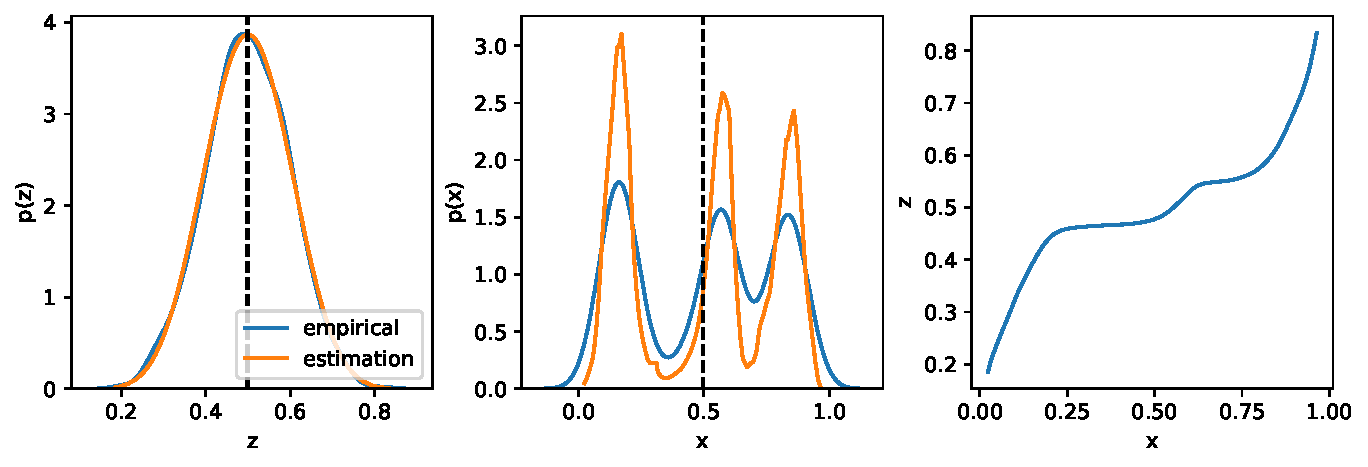
\includegraphics[width=\linewidth]{figures/1D/BLOBS/plot_1D.pdf}
      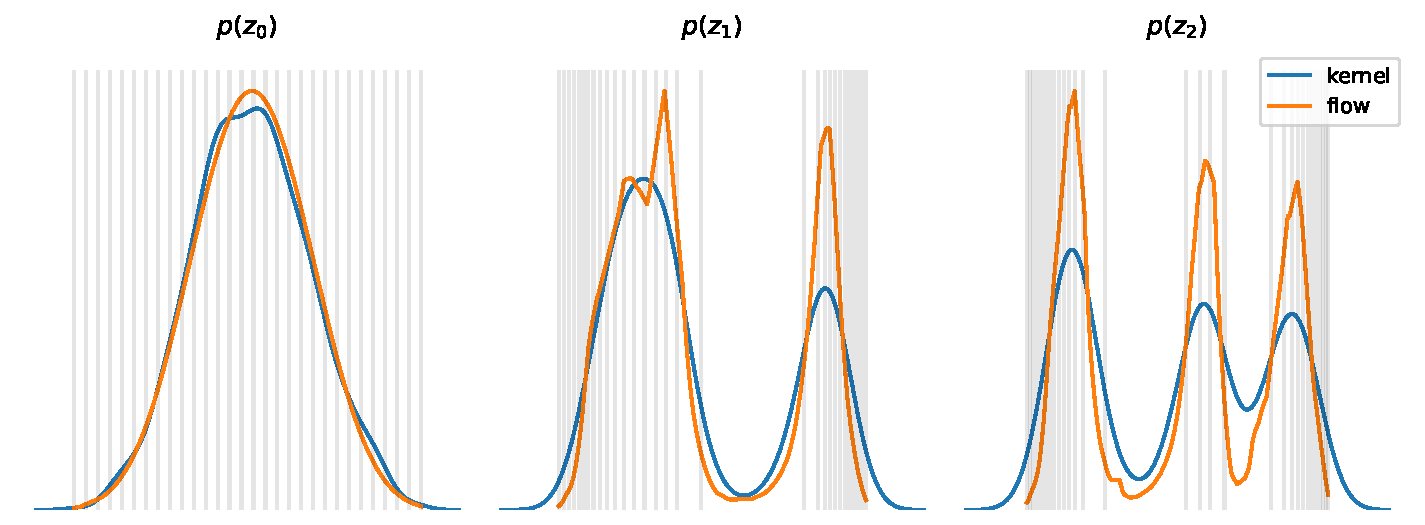
\includegraphics[width=\linewidth, trim=0 0 0 20, clip]{figures/1D/BLOBS/plot_generative_flow_evolution.pdf}
      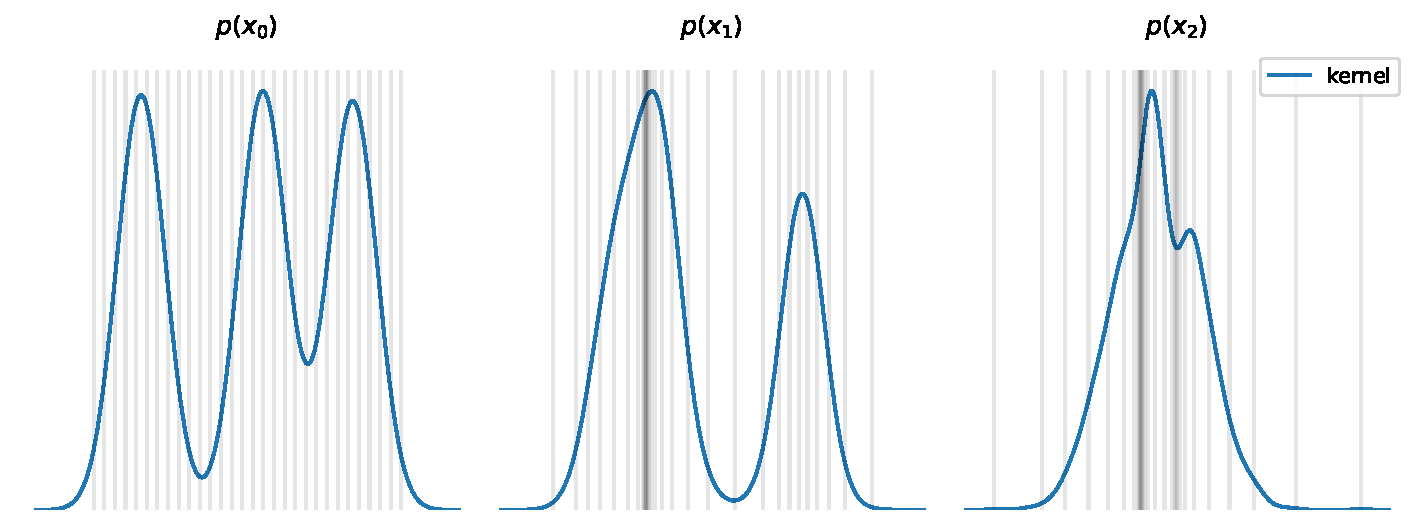
\includegraphics[width=\linewidth, trim=0 0 0 26, clip]{figures/1D/BLOBS/plot_normalizing_flow_evolution.pdf}
      \caption{\textsc{blobs} dataset}
      \label{fig:NF_1D_BLOBS}
    \end{subfigure}
    \hfill{\color{lightgray}\vrule}\hfill
    \begin{subfigure}[b]{0.48\linewidth}
      \centering
      % 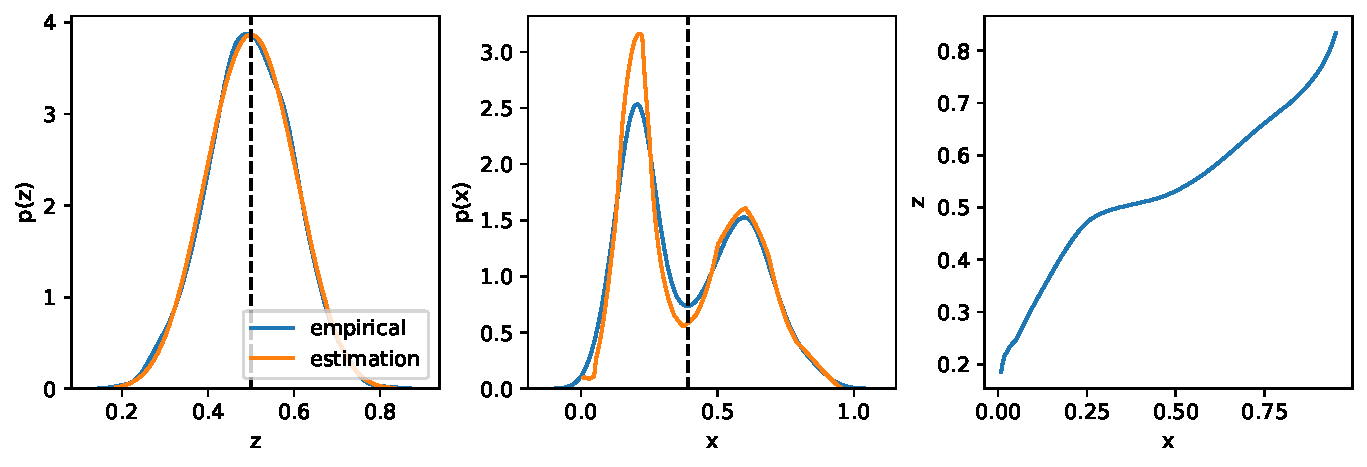
\includegraphics[width=\linewidth]{figures/1D/GAUSSIANMIXTURE/plot_1D.pdf}
      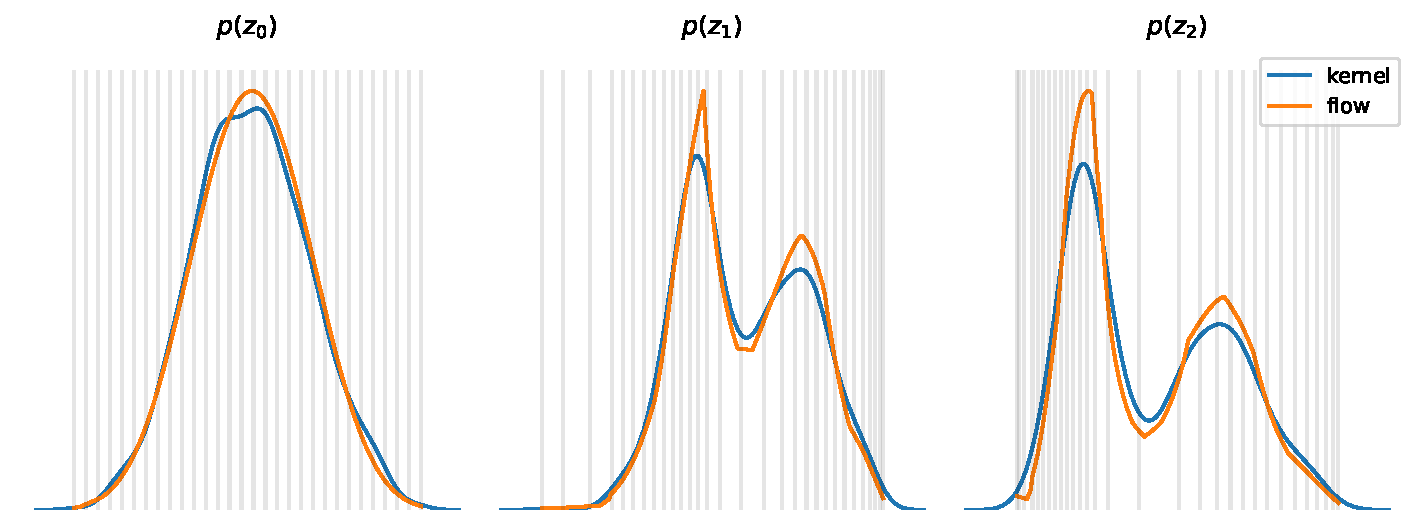
\includegraphics[width=\linewidth, trim=0 0 0 20, clip]{figures/1D/GAUSSIANMIXTURE/plot_generative_flow_evolution.pdf}
      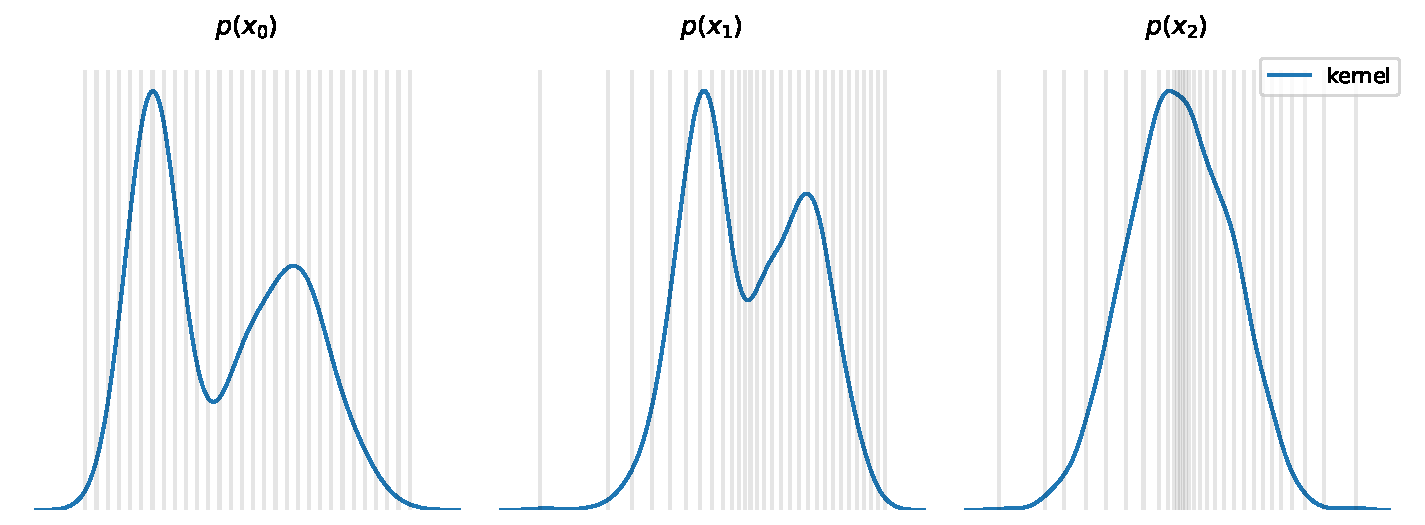
\includegraphics[width=\linewidth, trim=0 0 0 26, clip]{figures/1D/GAUSSIANMIXTURE/plot_normalizing_flow_evolution.pdf}
      \caption{\textsc{gaussianmix} dataset}
      \label{fig:NF_1D_GAUSSIANMIXTURE}
    \end{subfigure}
    \vspace{1em}
    \begin{subfigure}[b]{0.48\linewidth}
      \centering
      % 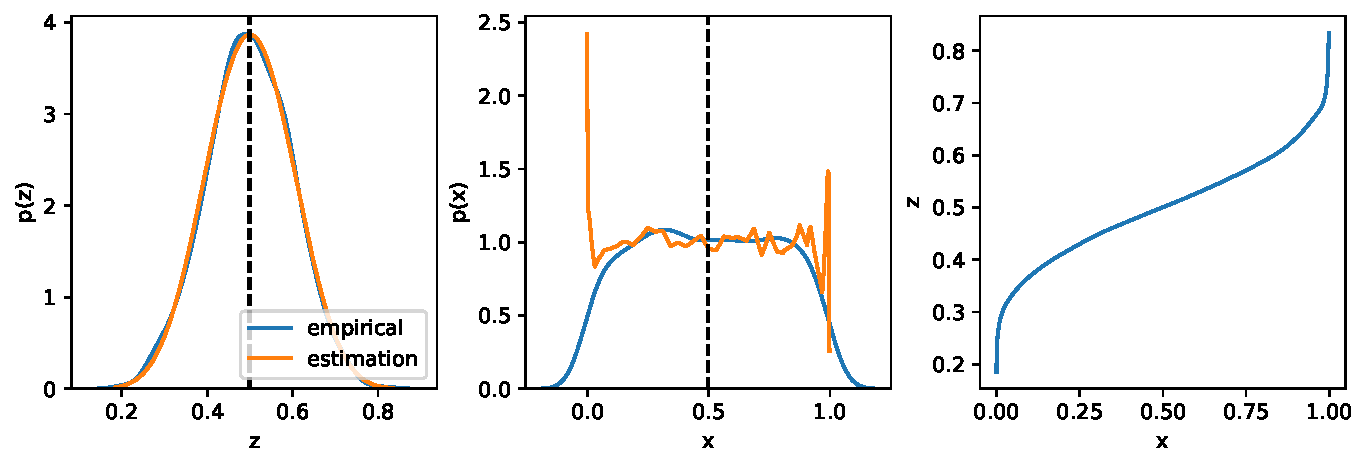
\includegraphics[width=\linewidth]{figures/1D/UNIFORM/plot_1D.pdf}
      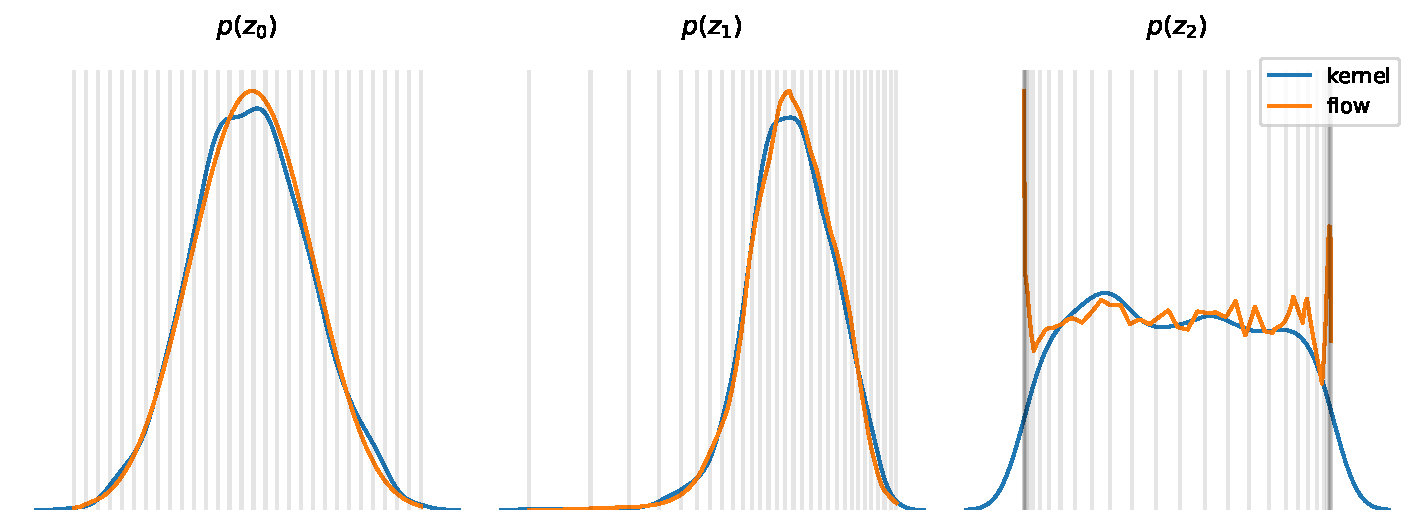
\includegraphics[width=\linewidth, trim=0 0 0 20, clip]{figures/1D/UNIFORM/plot_generative_flow_evolution.pdf}
      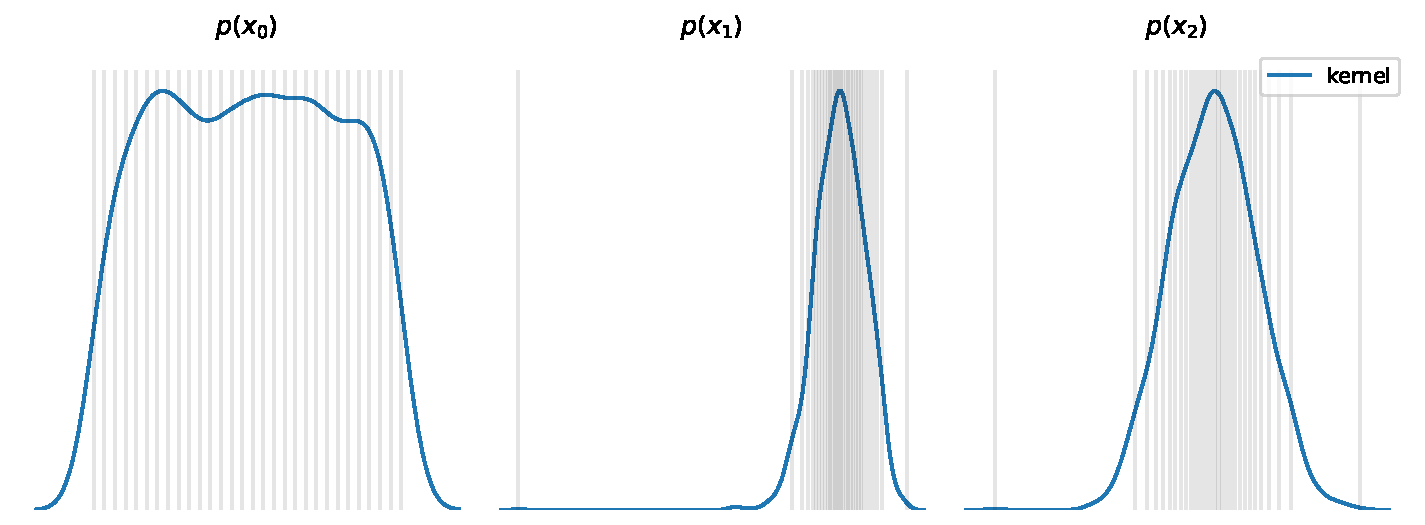
\includegraphics[width=\linewidth, trim=0 0 0 26, clip]{figures/1D/UNIFORM/plot_normalizing_flow_evolution.pdf}
      \caption{\textsc{uniform} dataset}
      \label{fig:NF_1D_UNIFORM}
    \end{subfigure}
    \hfill{\color{lightgray}\vrule}\hfill
    \begin{subfigure}[b]{0.48\linewidth}
      \centering
      % 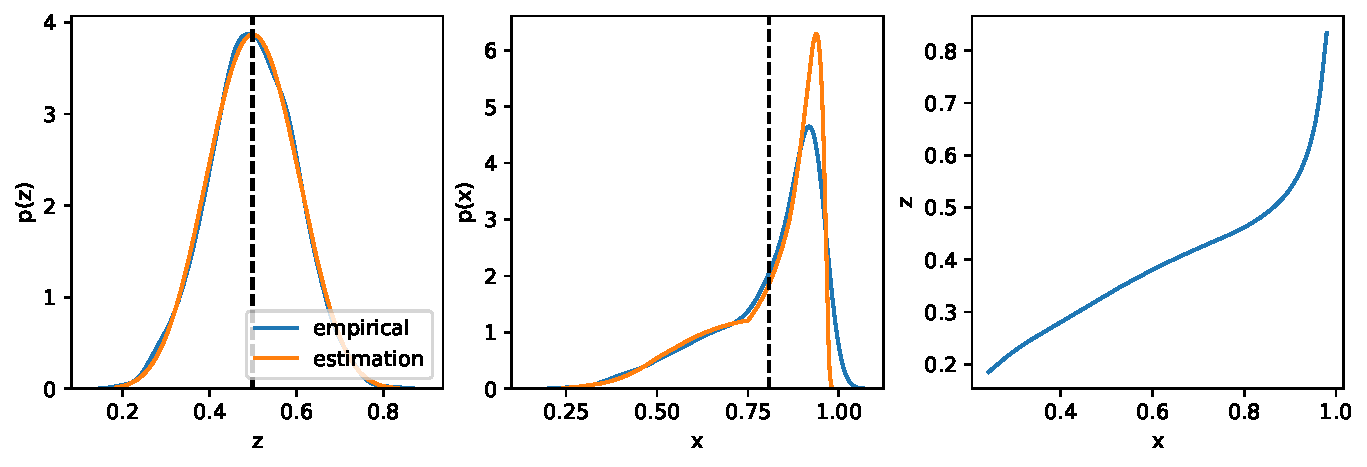
\includegraphics[width=\linewidth]{figures/1D/POWER/plot_1D.pdf}
      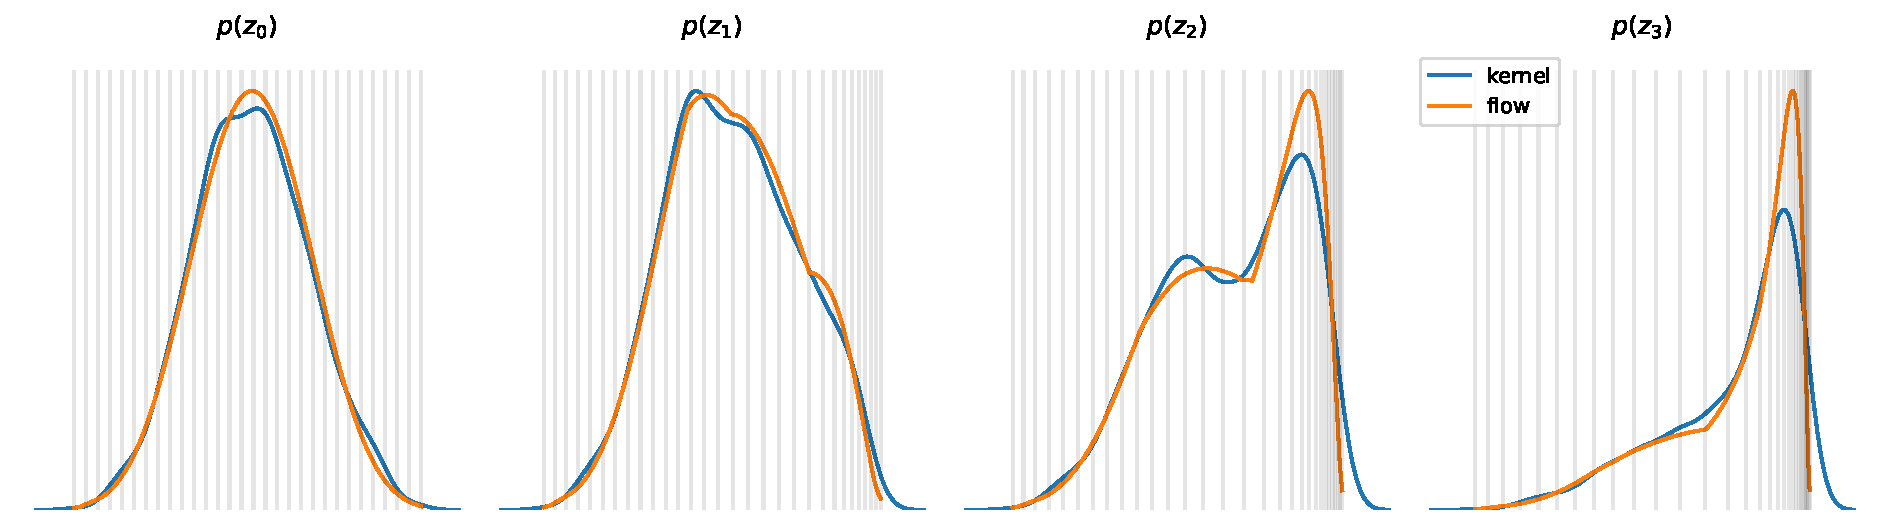
\includegraphics[width=\linewidth, trim=0 0 0 20, clip]{figures/1D/POWER/plot_generative_flow_evolution.pdf}
      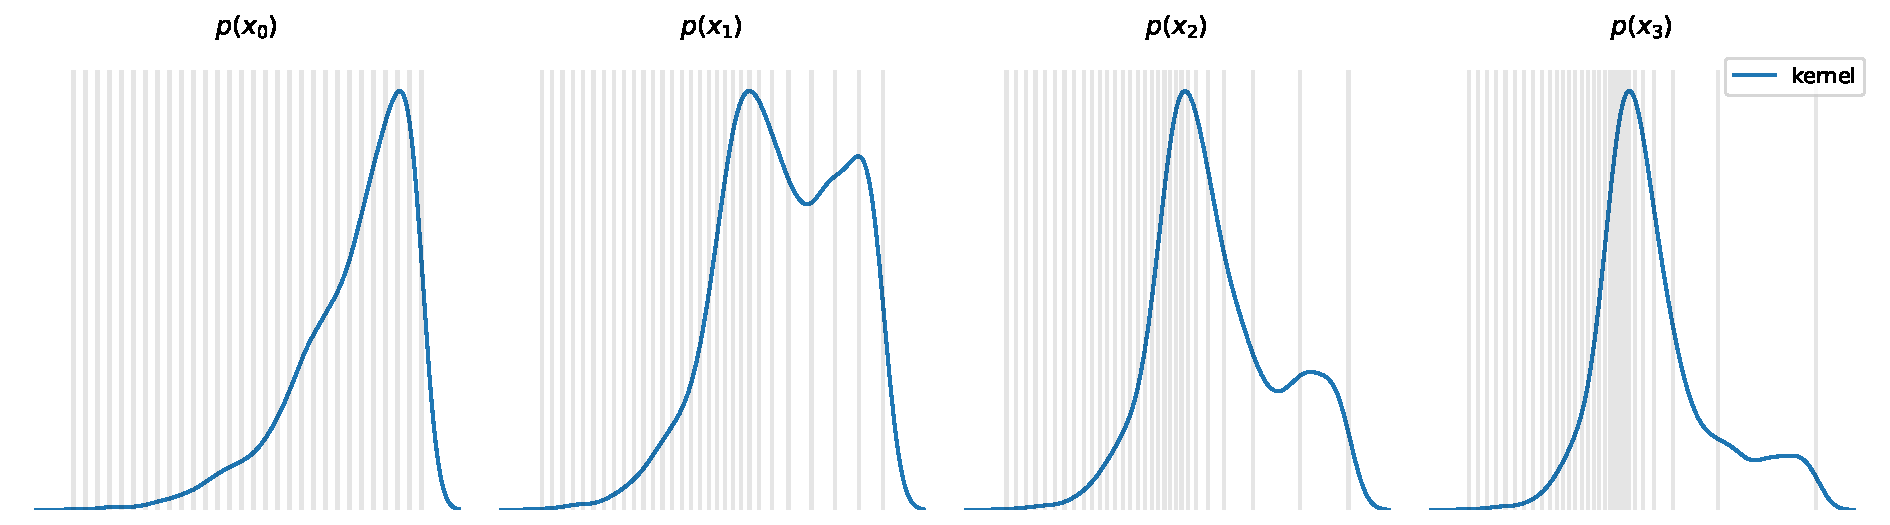
\includegraphics[width=\linewidth, trim=0 0 0 26, clip]{figures/1D/POWER/plot_normalizing_flow_evolution.pdf}
      \caption{\textsc{power} dataset}
      \label{fig:NF_1D_POWER}
    \end{subfigure}
    \caption{1D normalizing flows on multiple datasets. \textbf{Top}: Generative flow from Gaussian distribution to data. Kernel probability density estimate in \textcolor{blue}{blue} and inferred probability using the change-of-variable formula in \textcolor{orange}{orange}. \textbf{Bottom}: Normalizing flow from data back to the Gaussian distribution.}
    \label{fig:nf_1d_datasets}
  \end{center}
\end{figure}

\subsection{2-dimensional Data}

In this section the flexibility of DIFW-NF is demonstrated on synthetic two-dimensional datasets. A fully-connected neural network with ReLu activation function computes the parameters of the element-wise transformations.
A grid-hyperparameter search is conducted for each dataset. Flows can be composed after $1$,$2$,$3$,$4$ or $8$ steps and the transformation tessellation size is chosen among $\{4,8,16,32\}$.
In this case, a grid-search over network architectures was also performed; we searched over models with $1$,$2$ or $4$ layers with $8$ or $16$ hidden layers per flow.
The Adam optimizer \cite{kingma2014adam} is used with default hyperparameters and an initial learning rate of $1e^{-4}$ over $500$ training epochs with batch size $256$. For training and test, $5000$ and $2000$ data points are used respectively. 
The final hyperparameters are shown in \cref{tab:nf_2d}, along with the log-likelihood of the generated data.


\begin{table}[!htb]
  \small
  \caption{Hyperparameters and log-probability for density-estimation results in 2D-datasets}
  \label{tab:nf_2d}
  \vspace{-1em}
  \setstretch{0.87}
  \begin{center}
  \begin{tabular}{lccccl}
    \toprule
          Dataset & \begin{tabular}[c]{l}\# Neurons\\ per Layer\end{tabular} & \begin{tabular}[c]{l}\# Hidden\\Layers\end{tabular} & \begin{tabular}[c]{l}Tessellation\\Size $N_\mathcal{P}$\end{tabular} & \begin{tabular}[c]{l}Flow\\Steps\end{tabular} & $\log p(\mathbf{x})$ \\
    \midrule
               \textsc{abs} &                   16 &                1 &                32 &          2 &     -1.15 $\pm$ 0.06 \\
      \textsc{checkerboard} &                   16 &                4 &                32 &          1 &     -3.71 $\pm$ 0.06 \\
           \textsc{circles} &                   16 &                2 &                32 &          1 &     -1.24 $\pm$ 0.06 \\
          \textsc{crescent} &                   16 &                2 &                 4 &          1 &     -1.79 $\pm$ 0.06 \\
     \textsc{crescentcubed} &                    8 &                4 &                 4 &          1 &     -1.75 $\pm$ 0.09 \\
           \textsc{diamond} &                   16 &                4 &                32 &          1 &     -3.40 $\pm$ 0.06 \\
       \textsc{fourcircles} &                   16 &                4 &                 8 &          2 &     -2.90 $\pm$ 0.06 \\
             \textsc{moons} &                   16 &                4 &                32 &          2 &     -1.10 $\pm$ 0.06 \\
              \textsc{sign} &                   16 &                2 &                32 &          3 &     -1.43 $\pm$ 0.07 \\
          \textsc{sinewave} &                   16 &                2 &                32 &          3 &     -1.96 $\pm$ 0.05 \\
        \textsc{twospirals} &                   16 &                2 &                 4 &          8 &     -2.81 $\pm$ 0.05 \\
    \bottomrule
    \end{tabular}
  \end{center}
\end{table}


\begin{figure}[!htb]
    \begin{center}
      \begin{subfigure}{\linewidth}
          \centering
          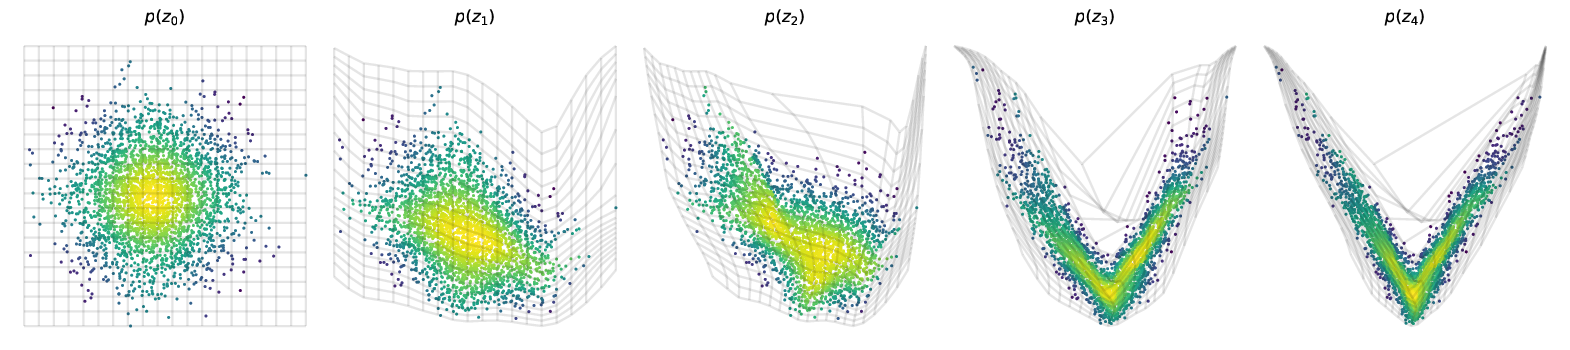
\includegraphics[width=0.75\linewidth,trim=0cm 0cm 0cm 1.6cm, clip]{figures/2D/ABS/plot_generative_flow_evolution.png}
          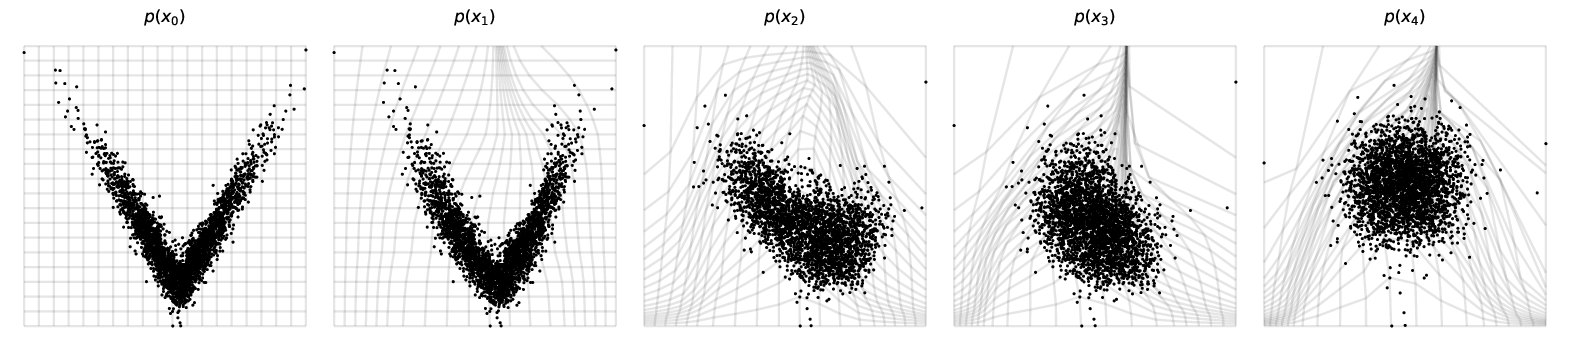
\includegraphics[width=0.75\linewidth,trim=0cm 0cm 0cm 1.6cm, clip]{figures/2D/ABS/plot_normalizing_flow_evolution.png}
          \caption{\textsc{abs} dataset}
          \label{fig:NF_2D_ABS}
      \end{subfigure}
      \vspace{1em}
      \begin{subfigure}{\linewidth}
        \centering
        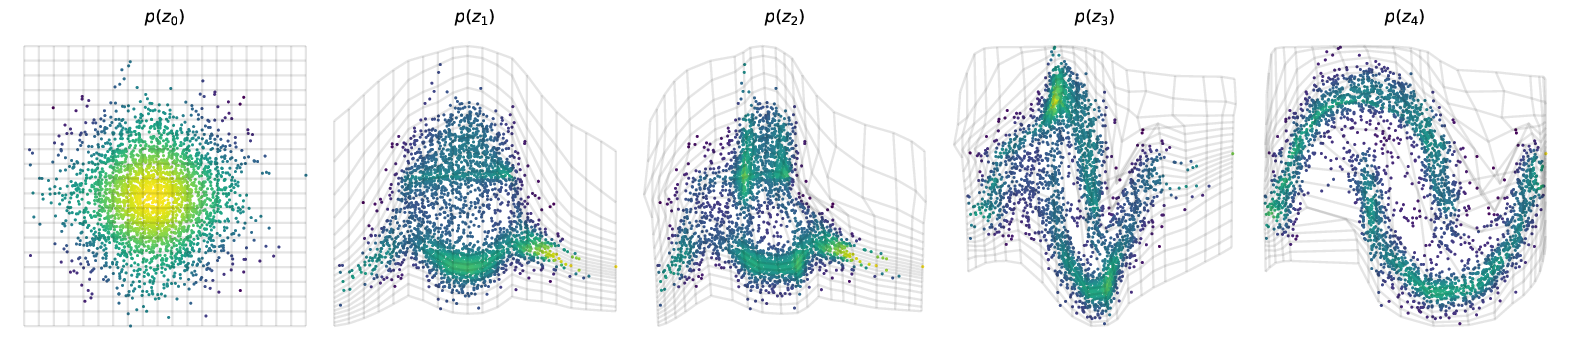
\includegraphics[width=0.75\linewidth,trim=0cm 0cm 0cm 1.6cm, clip]{figures/2D/MOONS/plot_generative_flow_evolution.png}
        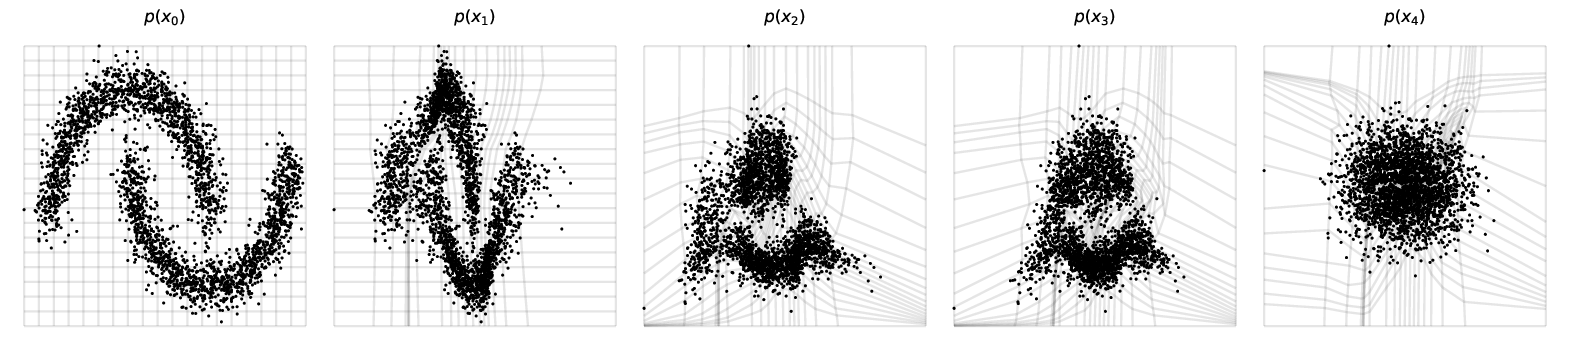
\includegraphics[width=0.75\linewidth,trim=0cm 0cm 0cm 1.6cm, clip]{figures/2D/MOONS/plot_normalizing_flow_evolution.png}
        \caption{\textsc{moons} dataset}
        \label{fig:NF_2D_MOONS}
      \end{subfigure}
    \caption{Density estimation for two-dimensional synthetic datasets, including multi-modal and discontinuous densities. Flow transforms samples from a standard-normal base density to the target density. The top row shows the generative direction, visualizing the transformation from noise to data: $\mathbf{z} \sim p(\mathbf{z}) \rightarrow \mathbf{x} = f(\mathbf{z})$. The color scale represents the probability density function. Normalizing flows are reversible, so one can train on a density estimation task and still be able to sample from the learned density efficiently. The bottom row shows the normalizing direction from data to noise: $\mathbf{x} \sim p(\mathbf{x}) \rightarrow \mathbf{z} = f^{-1}(\mathbf{x})$}
    \label{fig:nf_2d_examples:2}
  \end{center}
  \end{figure}
  


\begin{figure}[!htb]\ContinuedFloat
  \begin{center}
    \begin{subfigure}{\linewidth}
        \centering
        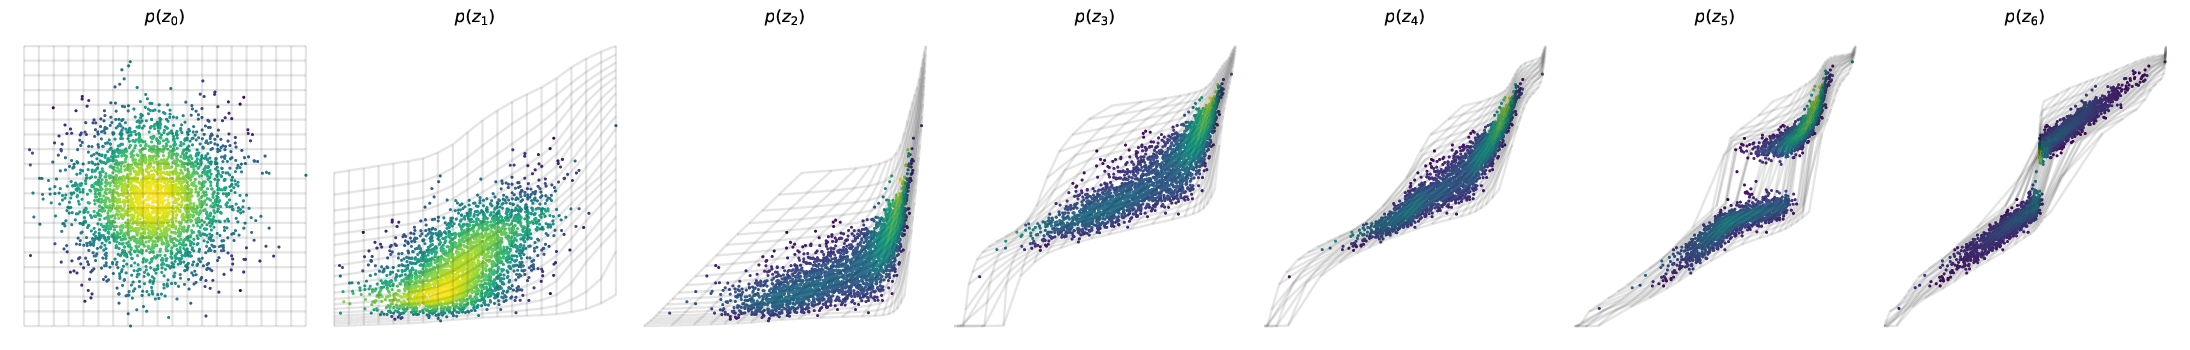
\includegraphics[width=\linewidth,trim=0cm 0cm 0cm 1.6cm, clip]{figures/2D/SIGN/plot_generative_flow_evolution.png}
        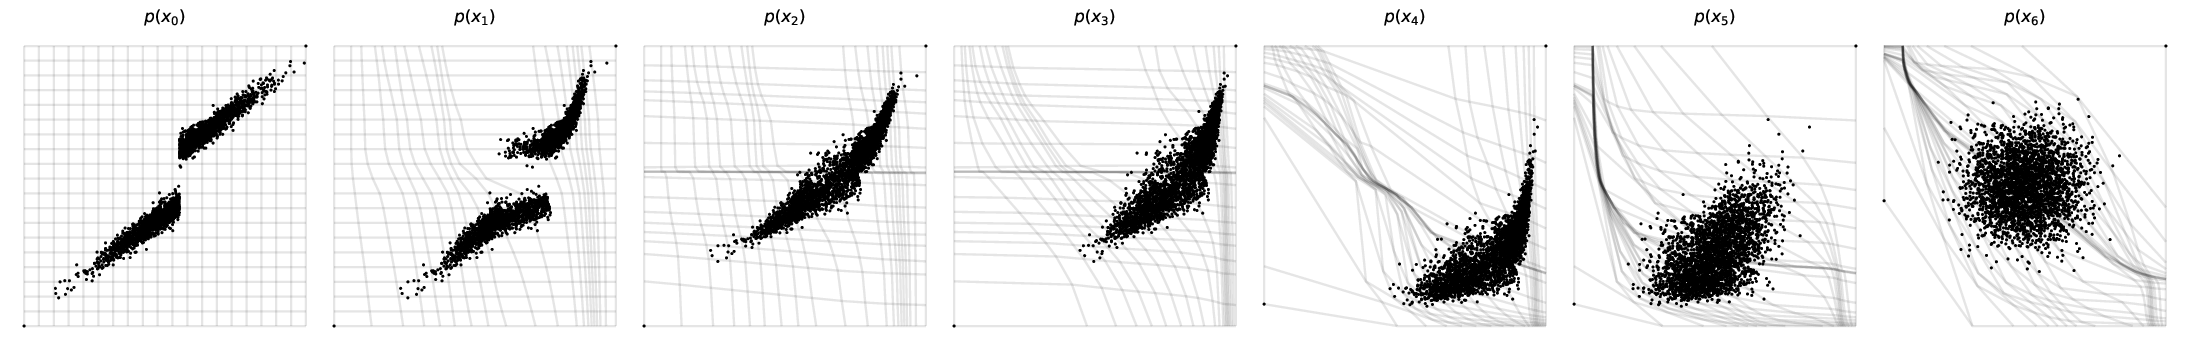
\includegraphics[width=\linewidth,trim=0cm 0cm 0cm 1.6cm, clip]{figures/2D/SIGN/plot_normalizing_flow_evolution.png}
        \caption{\textsc{sign} dataset}
        \label{fig:NF_2D_SIGN}
    \end{subfigure}
    \vspace{1em}
    \begin{subfigure}{\linewidth}
      \centering
      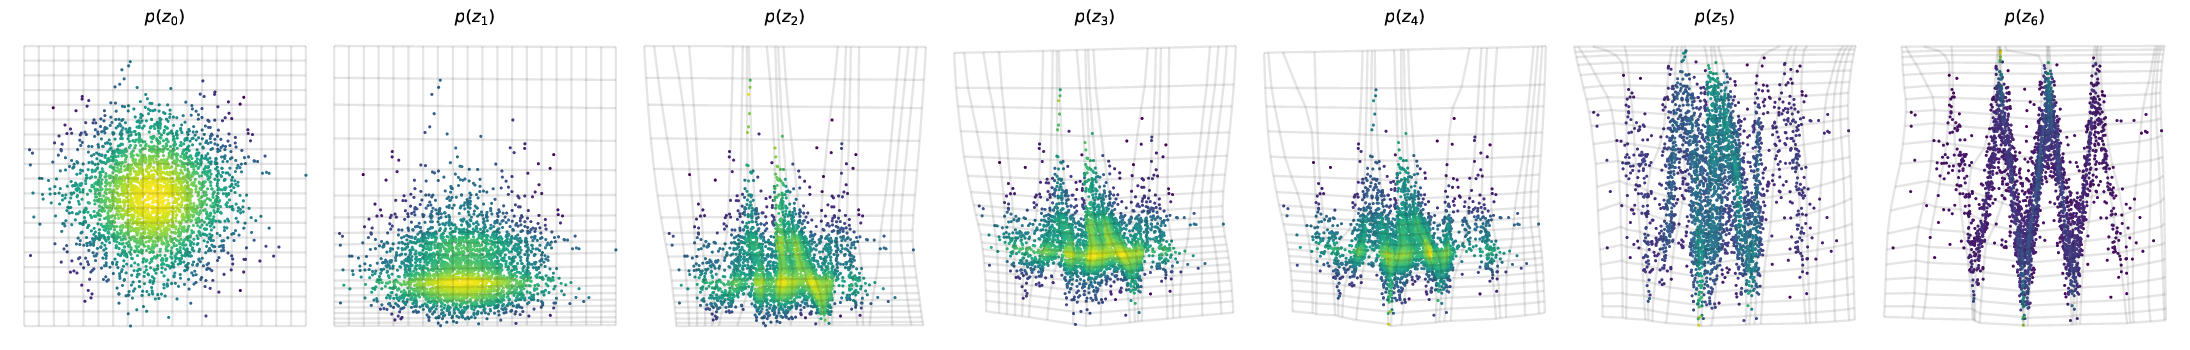
\includegraphics[width=\linewidth,trim=0cm 0cm 0cm 1.6cm, clip]{figures/2D/SINEWAVE/plot_generative_flow_evolution.png}
      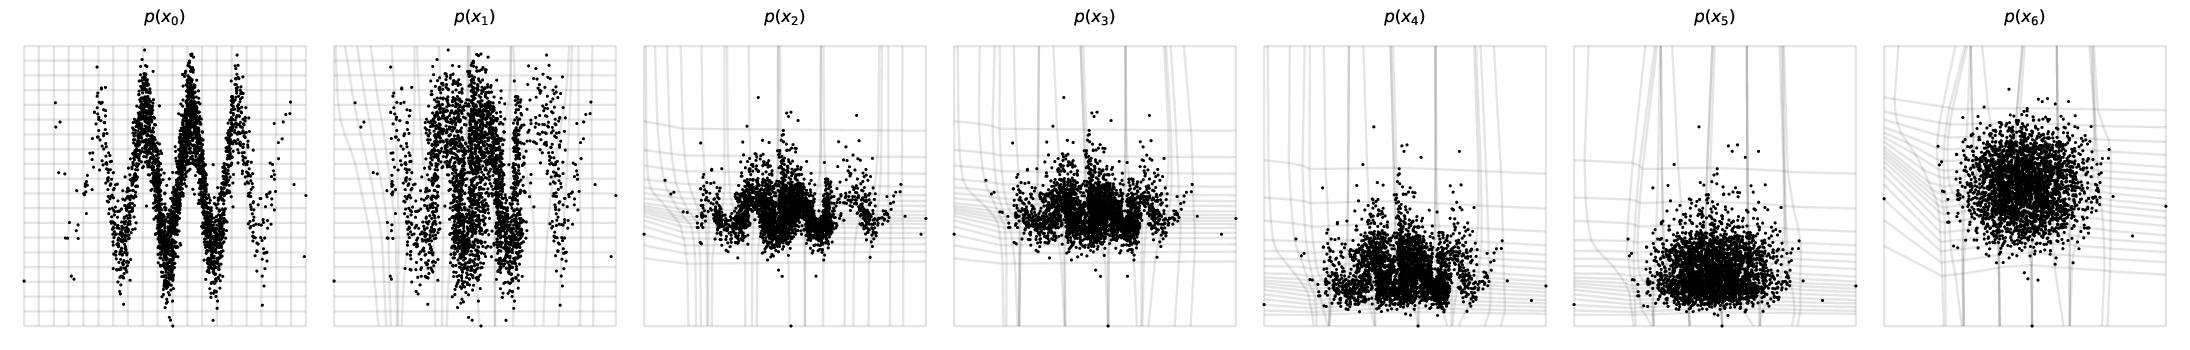
\includegraphics[width=\linewidth,trim=0cm 0cm 0cm 1.6cm, clip]{figures/2D/SINEWAVE/plot_normalizing_flow_evolution.png}
      \caption{\textsc{sinewave} dataset}
      \label{fig:NF_2D_SINEWAVE}
    \end{subfigure}
    \vspace{1em}
    \begin{subfigure}{\linewidth}
      \centering
      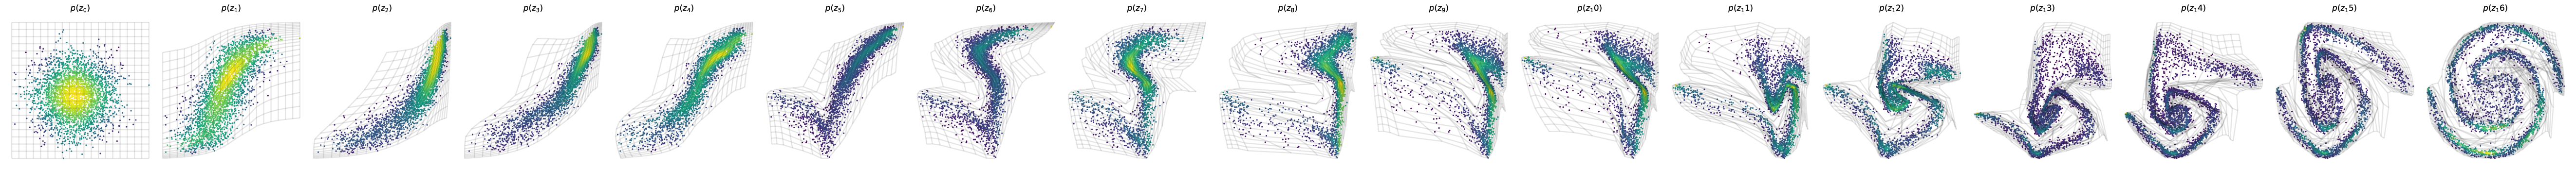
\includegraphics[width=\linewidth,trim=0cm 0cm 0cm 1.6cm, clip]{figures/2D/TWOSPIRALS/plot_generative_flow_evolution.png}
      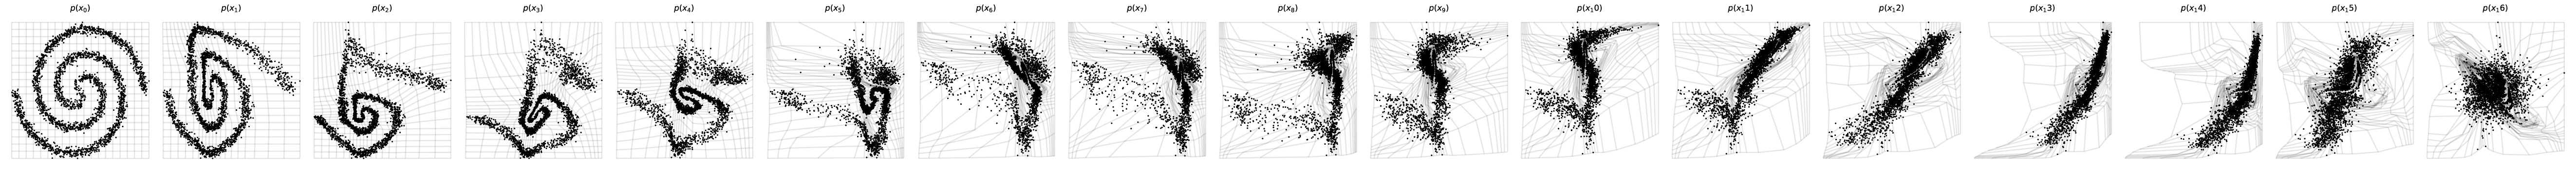
\includegraphics[width=\linewidth,trim=0cm 0cm 0cm 1.6cm, clip]{figures/2D/TWOSPIRALS/plot_normalizing_flow_evolution.png}
      \caption{\textsc{twospirals} dataset}
      \label{fig:NF_2D_TWOSPIRALS}
    \end{subfigure}
  \vspace{-2em}
  \caption{(Cont.) Density estimation for two-dimensional synthetic datasets, including multi-modal and discontinuous densities. Flow transforms samples from a standard-normal base density to the target density. The top row shows the generative direction, visualizing the transformation from noise to data: $\mathbf{z} \sim p(\mathbf{z}) \rightarrow \mathbf{x} = f(\mathbf{z})$. 
  The color scale represents the probability density function. 
  Normalizing flows are reversible, so one can train on a density estimation task and still be able to sample from the learned density efficiently. 
  The bottom row shows the normalizing direction from data to noise: $\mathbf{x} \sim p(\mathbf{x}) \rightarrow \mathbf{z} = f^{-1}(\mathbf{x})$.}
  \label{fig:nf_2d_examples:1}
\end{center}
\end{figure}

\begin{figure}[!htb]\ContinuedFloat
  \begin{center}
    \begin{subfigure}{0.48\linewidth}
      \centering
      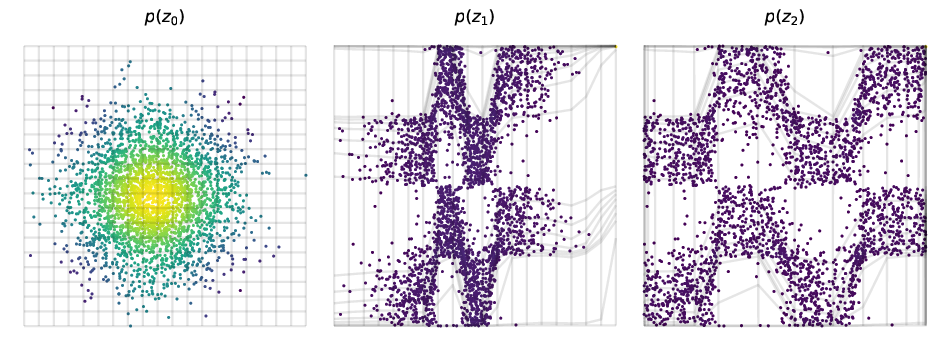
\includegraphics[width=\linewidth,trim=0cm 0cm 0cm 1.6cm, clip]{figures/2D/CHECKERBOARD/plot_generative_flow_evolution.png}
      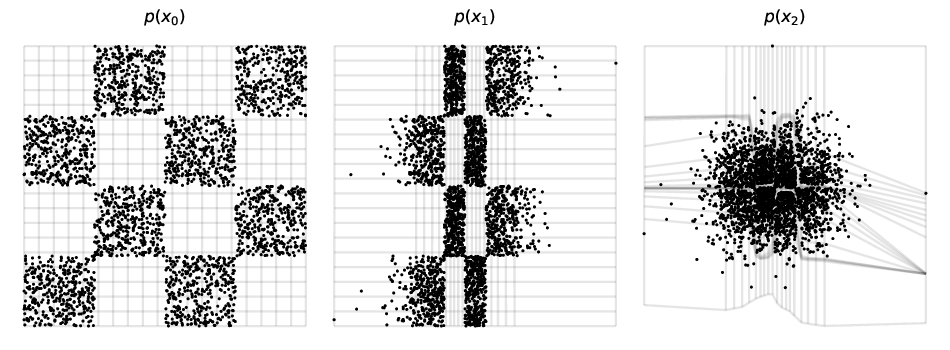
\includegraphics[width=\linewidth,trim=0cm 0cm 0cm 1.6cm, clip]{figures/2D/CHECKERBOARD/plot_normalizing_flow_evolution.png}
      \caption{\textsc{checkerboard} dataset}
      \label{fig:NF_2D_CHECKERBOARD}
    \end{subfigure}
    \hfill{\color{lightgray}\vrule}\hfill
    \begin{subfigure}{0.48\linewidth}
      \centering
      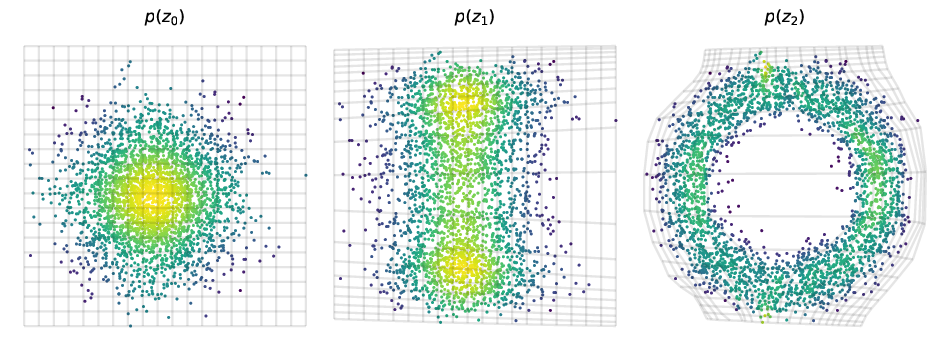
\includegraphics[width=\linewidth,trim=0cm 0cm 0cm 1.6cm, clip]{figures/2D/CIRCLES/plot_generative_flow_evolution.png}
      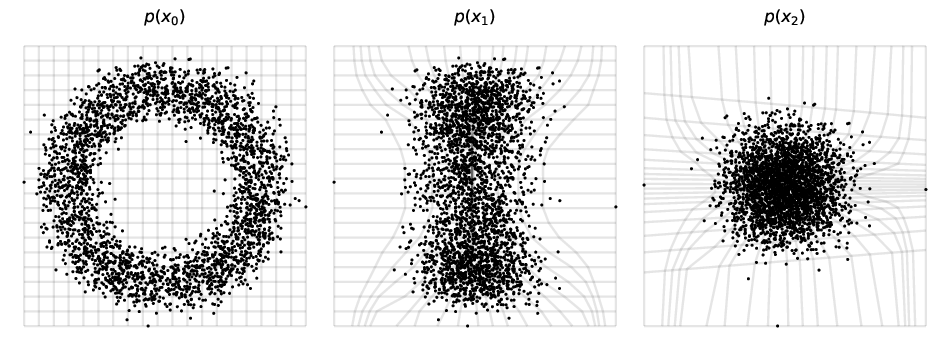
\includegraphics[width=\linewidth,trim=0cm 0cm 0cm 1.6cm, clip]{figures/2D/CIRCLES/plot_normalizing_flow_evolution.png}
      \caption{\textsc{circles} dataset}
      \label{fig:NF_2D_CIRCLES}
    \end{subfigure}
    \vspace{1em}
    \begin{subfigure}{0.48\linewidth}
      \centering
      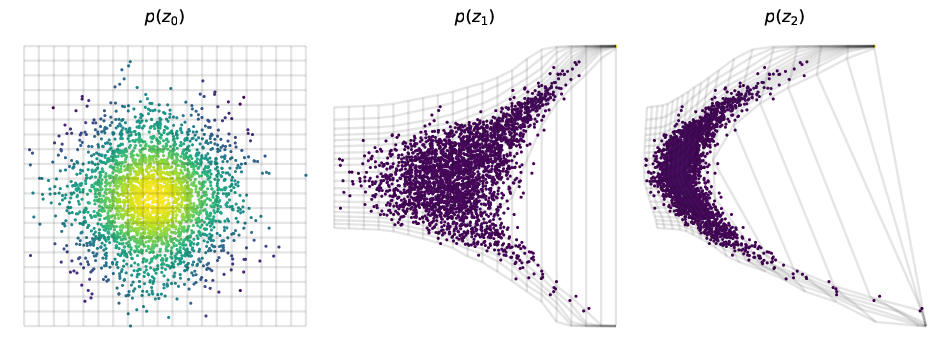
\includegraphics[width=\linewidth,trim=0cm 0cm 0cm 1.6cm, clip]{figures/2D/CRESCENT/plot_generative_flow_evolution.png}
      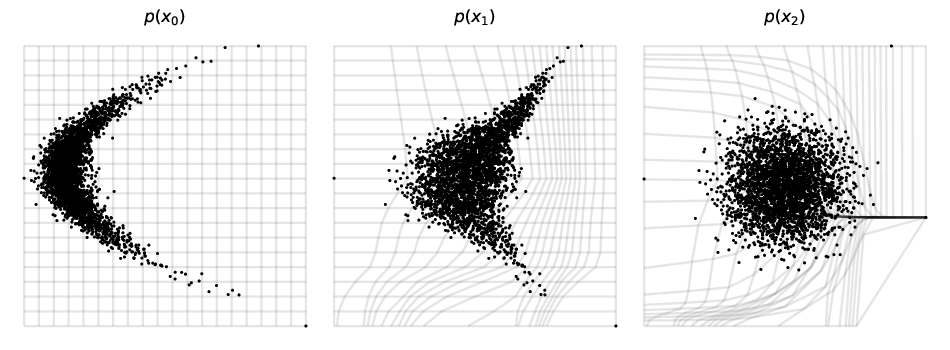
\includegraphics[width=\linewidth,trim=0cm 0cm 0cm 1.6cm, clip]{figures/2D/CRESCENT/plot_normalizing_flow_evolution.png}
      \caption{\textsc{crescent} dataset}
      \label{fig:NF_2D_CRESCENT}
    \end{subfigure}
    \hfill{\color{lightgray}\vrule}\hfill
    \begin{subfigure}{0.48\linewidth}
      \centering
      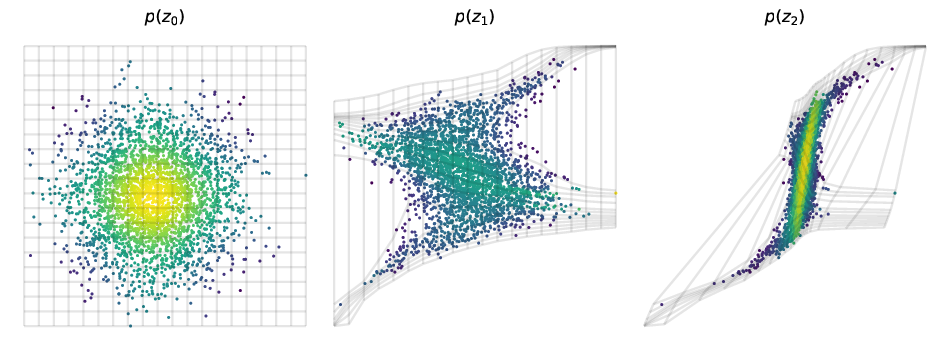
\includegraphics[width=\linewidth,trim=0cm 0cm 0cm 1.6cm, clip]{figures/2D/CRESCENTCUBED/plot_generative_flow_evolution.png}
      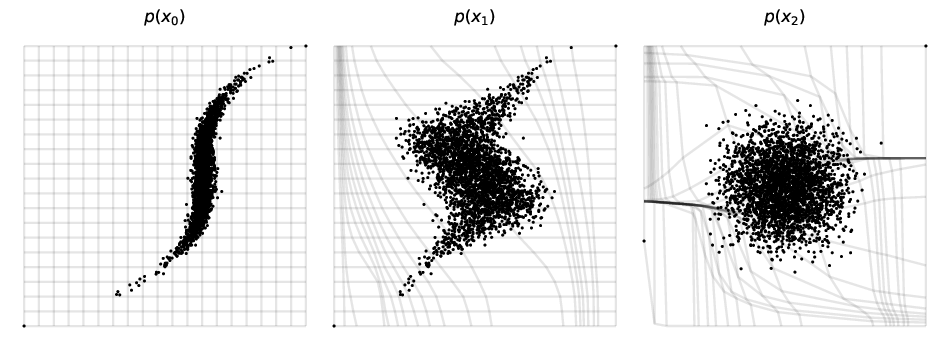
\includegraphics[width=\linewidth,trim=0cm 0cm 0cm 1.6cm, clip]{figures/2D/CRESCENTCUBED/plot_normalizing_flow_evolution.png}
      \caption{\textsc{crescentcubed} dataset}
      \label{fig:NF_2D_CRESCENTCUBED}
    \end{subfigure}
    \caption{(Cont.) Density estimation for two-dimensional synthetic datasets, including multi-modal and discontinuous densities. Flow transforms samples from a standard-normal base density to the target density. The top row shows the generative direction, visualizing the transformation from noise to data: $\mathbf{z} \sim p(\mathbf{z}) \rightarrow \mathbf{x} = f(\mathbf{z})$. The color scale represents the probability density function. Normalizing flows are reversible, so one can train on a density estimation task and still be able to sample from the learned density efficiently. The bottom row shows the normalizing direction from data to noise: $\mathbf{x} \sim p(\mathbf{x}) \rightarrow \mathbf{z} = f^{-1}(\mathbf{x})$}
    \label{fig:nf_2d_examples:3}
  \end{center}
\end{figure}

\cref{fig:nf_2d_examples:1,fig:nf_2d_examples:2,fig:nf_2d_examples:3} shows qualitative results for two-dimensional synthetic datasets. The comparison of the generated points with the original data shows that the normalizing flows can accurately replicate multi-modal and discontinuous distributions. DIFW-NF is able to achieve this with a limited number of flow layers and small neural network architecture, i.e., small number of hidden layers and neurons per layer. 
It is worth noting that the \textsc{twospirals} dataset, which has a complex and non-linear distribution, requires more than three flow steps to generate accurate results. Considering other models, comparisons are avoided in this instance because these datasets are small, simple and not representative of real-world data. Models that perform well on toy datasets may not necessarily perform well on larger, more complex datasets. Hence, the next section focuses on experiments on N-dimensional real-world data. 

\subsection{N-dimensional Data}

We evaluate our proposed flows using a selection of datasets from the UCI machine-learning
repository \cite{asuncion2007uci} and BSDS300 collection of natural images \cite{martin2001database}. This is the standard suite of benchmarks for density estimation of tabular data. The experimental setup and pre-processing of \cite{papamakarios2017masked} is followed, who make their data available online.

Model selection is performed using the standard validation splits for these datasets. The norm of gradients is clipped to the range $[-5, 5]$, and find this helps stabilize training. 
In this case a fully-connected neural network of $4$ layers with $64$ neurons per layer with ReLu activation function was chosen to compute the parameters of the element-wise transformations. A grid-search is not carried out to optimize the neural network architecture.

On the contrary, a grid-hyperparameter search is conducted for the transformation of each dataset. Flows can be composed after $3$,$5$,$8$,$10$,$15$ or $20$ steps and the transformation tessellation size is chosen among $\{5,10,20,50\}$.
In addition, a grid-search over network architectures was also performed; we searched over models with $1$,$2$ or $4$ layers with $8$ or $16$ hidden layers per flow.
The Adam optimizer \cite{kingma2014adam} was used with default hyperparameters and an initial learning rate of $3e^{-4}$ or $5e^{-4}$ over $128$, $256$ or $512$ training epochs with batch size $512$. 

Hyperparameter settings are shown for coupling flows in \cref{tab:nf_nd}. The dimensionality and number of training data points are included in each table for reference. 
%For higher dimensional datasets such as Hepmass and BSDS300, we found increasing the number of flow layers beneficial. This was not necessary for Miniboone, where overfitting was an issue due to the low number of data points.
\begin{table}[!htb]
  \small
  \caption{Hyperparameters and log-probability for density-estimation results in ND-datasets}
  \label{tab:nf_nd}
  \vspace{-1em}
  \begin{center}
  \begin{tabular}{llllllll}
    \toprule
    Dataset &  \textsc{bsds}\footnotesize300 & \textsc{gas} & \textsc{hepmass} & \textsc{miniboone} & \textsc{power} \\
    \midrule
    Train Points         &  1000000 &  852174 &  315123 &     29556 &  1615917  \\
    Dimension            &       63 &       8 &      21 &        43 &        6  \\
    \midrule
    Batch Size           &      512 &     512 &     512 &       512 &      512  \\
    \# Neurons per Layer &       64 &      64 &      64 &        64 &       64  \\
    \# Hidden Layers     &        4 &       4 &       4 &         4 &        4  \\
    Tessellation Size    &       10 &      10 &      10 &        10 &       50  \\
    Flow Steps           &       15 &      15 &      10 &        10 &        3  \\
    Epochs               &      256 &     256 &     256 &       512 &      128  \\
    Learning Rate        &   0.0005 &  0.0005 &  0.0005 &    0.0003 &   0.0005  \\
    \bottomrule
  \end{tabular}
\end{center}
\end{table}

\vspace{-0.5cm}
\begin{table}[!htb]
  \small
  \caption{Test log-likelihood (in nats) for UCI datasets and BSDS300, with error bars corresponding to two standard deviations. Higher is better.}
  \label{tab:nf_nd_results}
  \vspace{-1em}
  \begin{center}
  \begin{tabular}{llllll}
    \toprule
    Dataset &  \textsc{bsds300} & \textsc{gas} & \textsc{hepmass} & \textsc{miniboone} & \textsc{power} \\
    \midrule
    DIFW (AR)    &  155.95 $\pm$ 0.39 &  11.60 $\pm$ 0.02 &  -14.18 $\pm$ 0.04 &   -9.06 $\pm$ 0.07 &  0.45 $\pm$ 0.01 \\
    DIFW (CL)    &  \textbf{160.25} $\pm$ 0.40 &  10.79 $\pm$ 0.03 &  -15.32 $\pm$ 0.03 &   \textbf{-8.02} $\pm$ 0.06 &  0.30 $\pm$ 0.01 \\
    BLOCK-NAF    &  157.36 $\pm$ 0.03 &  12.06 $\pm$ 0.09 &  -14.71 $\pm$ 0.38 &   -8.95 $\pm$ 0.07 &  0.61 $\pm$ 0.01 \\
    FFJORD       &  157.40 $\pm$ 0.19 &   8.59 $\pm$ 0.12 &  -14.92 $\pm$ 0.08 &  -10.43 $\pm$ 0.04 &  0.46 $\pm$ 0.01 \\
    GLOW         &  156.95 $\pm$ 0.28 &  12.24 $\pm$ 0.03 &  -16.99 $\pm$ 0.02 &  -10.55 $\pm$ 0.45 &  0.52 $\pm$ 0.01 \\
    MAF          &  156.95 $\pm$ 0.28 &  12.35 $\pm$ 0.02 &  -17.03 $\pm$ 0.02 &  -10.92 $\pm$ 0.46 &  0.45 $\pm$ 0.01 \\
    NAF          &  157.73 $\pm$ 0.04 &  11.96 $\pm$ 0.33 &  -15.09 $\pm$ 0.40 &   -8.86 $\pm$ 0.15 &  0.62 $\pm$ 0.01 \\
    Q-NSF (AR)   &  157.42 $\pm$ 0.28 &  12.91 $\pm$ 0.02 &  -14.67 $\pm$ 0.03 &   -9.72 $\pm$ 0.47 &  \textbf{0.66} $\pm$ 0.01 \\
    Q-NSF (C)    &  157.65 $\pm$ 0.28 &  12.80 $\pm$ 0.02 &  -15.35 $\pm$ 0.02 &   -9.35 $\pm$ 0.44 &  0.64 $\pm$ 0.01 \\
    RQ-NSF (AR)  &  157.31 $\pm$ 0.28 &  \textbf{13.09} $\pm$ 0.02 &  \textbf{-14.01} $\pm$ 0.03 &   -9.22 $\pm$ 0.48 &  \textbf{0.66} $\pm$ 0.01 \\
    RQ-NSF (C)   &  157.54 $\pm$ 0.28 &  \textbf{13.09} $\pm$ 0.02 &  -14.75 $\pm$ 0.03 &   -9.67 $\pm$ 0.47 &  0.64 $\pm$ 0.01 \\
    SOS          &  157.48 $\pm$ 0.41 &  11.99 $\pm$ 0.41 &  -15.15 $\pm$ 0.10 &   -8.90 $\pm$ 0.11 &  0.60 $\pm$ 0.01 \\\bottomrule
  \end{tabular}
\end{center}
\end{table}
\footnotetext{The average log-likelihood (relative entropy) is usually reported in units of nats. When one uses the natural logarithm to compute entropy, it takes on the "natural units of information", or nats.}

\begin{figure}[!htb]
  \begin{center}
  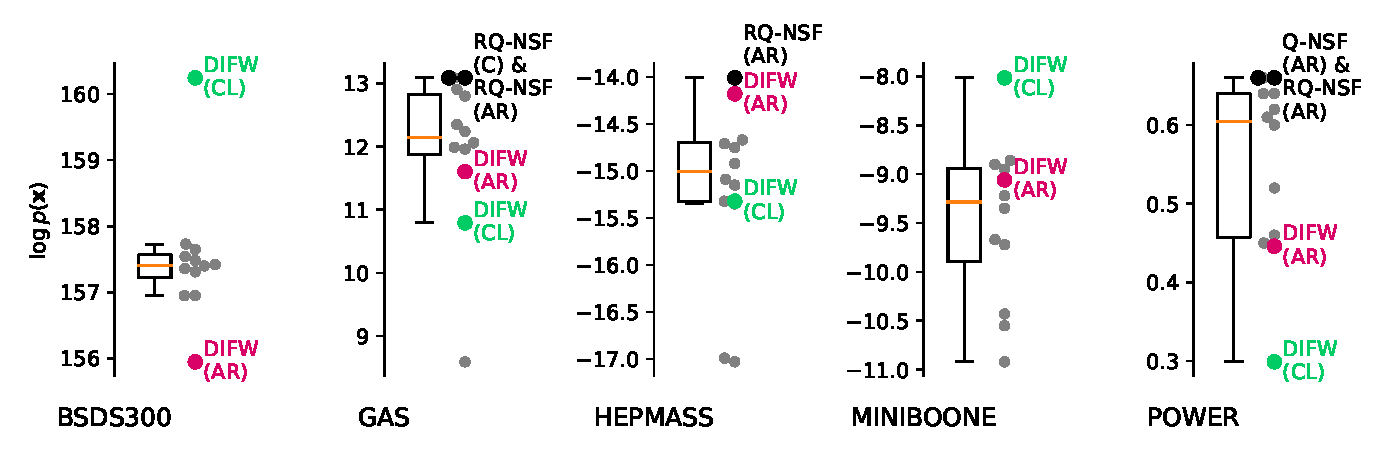
\includegraphics[width=\linewidth]{figures/ND/resultsND_boxplot2.pdf}
  \vspace{-0.8cm}
  \caption{Boxplot visualization. Each point represents the test log-likelihood (in nats) of each model for UCI datasets and BSDS300, higher is better.}
  \label{fig:nf_nd_results}
  \end{center}
\end{figure}

% In our experiments, the neural network which computes the parameters of the element-wise transformations is a
% We first evaluate our proposed flows using a selection of datasets from the UCI machine-learning repository [REF] and BSDS300 collection of natural images [REF]. 
% FIGURE: Validation log likelihood (in nats) for UCI datasets and BSDS300, with error bars corresponding to two standard deviations.
% \footnote{
%   The average log-likelihood (relative entropy) is usually reported in units of nats. hen we use the natural logarithm to compute entropy, it takes on the "natural units of information", or nats.
% }
% The average log-likelihood (relative entropy) is usually reported in units of nats. Shannon's Source Coding Theorem (1948) tells us that entropy H(p) is the lower bound on average code length for any code you can construct to communicate samples from p(x) losslessly. More entropy means more "randomness", which cannot be compressed. In particular, 

Our results are shown in \cref{tab:nf_nd_results,fig:nf_nd_results}.
DIFW (CL) achieve state-of-the-art results for \textsc{bsds300} and \textsc{miniboone}, while Both RQ-NSF (C) and RQ-NSF (AR) do so on the \textsc{power}, \textsc{gas}, and \textsc{hepmass} datasets, tied with Q-NSF (AR) on the \textsc{power} dataset. Moreover, DIFW (CL) and DIFW (AR) achieve competitive scores with the best autoregressive models (Glow and FFJORD). These results close the gap between autoregressive flows and flows based on coupling layers, and demonstrate that, in some cases, it may not be necessary to sacrifice one-pass sampling for density-estimation performance.
% For tabular density estimation, both RQ-NSF (C) and RQ-NSF (AR) excel on Power, Gas, and Hepmass, the datasets with the highest ratio of data points to dimensionality from the five considered.

\section{Conclusions}\label{sec:conclusions_6}

On the whole, DIFW-NF shows that upgrading the commonly-used affine transformations in coupling and autoregressive layers can significantly improve performance without compromising analytic invertibility. Through the use of monotonic transforms based on the integration of continuous piecewise-affine velocity functions, coupling-layer-based models can achieve density-estimation performance on par with the best autoregressive flows while maintaining exact one-pass sampling. These models find a unique compromise between versatility and flexibility, serving as a powerful off-the-shelf tool for enhancing architectures like the variational autoencoder and boosting parameter efficiency in generative modeling.

The proposed transforms scale to high-dimensional problems, as demonstrated empirically in \cref{sec:results_6}.
Moreover, due to the increased flexibility of the proposed transformations, it requires fewer steps to build flexible flows, reducing the computational cost. %In our experiments, we found rational-quadratic splines added approximately 30-40\% to the wall-clock time for a single traning update compared to the same model with affine transformations. 
A potential drawback of the proposed method is a more involved implementation. This is alleviated by providing an extensive \cref{sec:method_6} with technical details, and a reference implementation in PyTorch.

The proposed transformations are also a useful differentiable and invertible module in their own right, which could be included in many models that can be trained end-to-end. For instance, monotonic warping functions with a tractable Jacobian determinant are useful for supervised learning. More generally, invertibility can be useful for training very large networks, since activations can be recomputed on-the-fly for backpropagation, meaning gradient computation requires memory which is constant instead of linear in the depth of the network.
Monotonic transforms based on the integration of continuous piecewise-affine velocity functions are one way of constructing invertible element-wise transformations, but there may be others. The benefits of research in this direction are clear, and so we look forward to future work in this area.
